% Source formatting: one sentence per source line (semantic line breaks); preserve math syntax, environments, commands, and blank paragraph boundaries.
% L4DC/PMLR mathematical draft. All body, proofs, figure data, and references are here.
% Supporting results and complete proofs are integrated below and in the appendices.
% Complete conference paper with self-contained proofs and figure data.
\documentclass{l4dc2027}
\usepackage[T1]{fontenc}
\usepackage{times}
\usepackage{amsmath,amssymb,booktabs,mathrsfs}
\usepackage{graphicx}
\usepackage{tikz}
\usetikzlibrary{arrows.meta}
\newcommand{\R}{\mathbb R}
\providecommand{\todo}[1]{\textcolor{red}{[#1]}}
\newcommand{\eqdef}{\triangleq}
\makeatletter\@ifundefined{convention}{\newtheorem{convention}{Convention}}{}\makeatother
\makeatletter\@ifundefined{definition}{\newtheorem{definition}{Definition}}{}\makeatother
\makeatletter\@ifundefined{assumption}{\newtheorem{assumption}{Assumption}}{}\makeatother
\makeatletter\@ifundefined{lemma}{\newtheorem{lemma}{Lemma}}{}\makeatother
\makeatletter\@ifundefined{proposition}{\newtheorem{proposition}{Proposition}}{}\makeatother
\makeatletter\@ifundefined{corollary}{\newtheorem{corollary}{Corollary}}{}\makeatother
\makeatletter\@ifundefined{theorem}{\newtheorem{theorem}{Theorem}}{}\makeatother
\makeatletter\@ifundefined{example}{\newtheorem{example}{Example}}{}\makeatother
\makeatletter\@ifundefined{problem}{\newtheorem{problem}{Problem}}{}\makeatother
\makeatletter\@ifundefined{remark}{\newtheorem{remark}{Remark}}{}\makeatother
\makeatletter\@ifundefined{trainingalgorithm}{\newtheorem{trainingalgorithm}{Algorithm}}{}\makeatother
% Keep theorem and supporting-environment numbering independent.
\newtheorem{paperconvention}{Convention}
\let\convention\paperconvention
\let\endconvention\endpaperconvention
\newtheorem{paperdefinition}{Definition}
\let\definition\paperdefinition
\let\enddefinition\endpaperdefinition
\newtheorem{paperlemma}{Lemma}
\let\lemma\paperlemma
\let\endlemma\endpaperlemma
\newtheorem{paperproposition}{Proposition}
\let\proposition\paperproposition
\let\endproposition\endpaperproposition
\newtheorem{papercorollary}{Corollary}
\let\corollary\papercorollary
\let\endcorollary\endpapercorollary
\newtheorem{paperremark}{Remark}
\let\remark\paperremark
\let\endremark\endpaperremark

\title[Learning nonlinear predictors with certified stable reductions]{Learning Nonlinear Predictors with Certified Stable Reductions}
\author[Brown et~al.]{%
\Name{Brian Charles Brown}$^1$\quad
\Name{David Grimsman}$^1$\quad
\Name{Michael King}$^1$\\
\Name{Abel Palmer}$^1$\quad
\Name{Sean Warnick}$^1$\quad
\Name{Enoch Yeung}$^2$\\
\addr $^1$Department of Computer Science, Brigham Young University, Provo, UT, USA\\
\addr $^2$Department of Mechanical Engineering, University of California, Santa Barbara, CA, USA
}
% Abel Palmer is affiliated with BYU here because that is where he performed this work.
\AtBeginEnvironment{definition}{\normalfont}
\AtBeginEnvironment{proof}{\normalfont}
\AtBeginEnvironment{remark}{\normalfont}
% Compact links from supplementary results to their Lean declarations.
\newcommand{\leanref}[3]{\par\noindent{\scriptsize\textrm{Lean counterpart of #1}\enspace\IfFileExists{../lean/#2}{\href{https://github.com/Populustremuloides/certified-nonlinear-reduction/blob/main/lean/#2}{\texttt{\detokenize{#3}}}}{\texttt{\detokenize{#3}} (archived instance proof)}}\par}

\begin{document}
\maketitle
\begin{abstract}
Reducing the state dimension of a data-driven representation of a non-affine control system can make the representation unstable for some inputs, and no finite set of simulations can certify global asymptotic stability of an equilibrium.
Stability must therefore be derived from the representation itself, which is often difficult in data-driven settings.
We propose a representation for a large class of non-affine control systems that sums a stable linear Koopman model of the unforced dynamics with affine inputs comprising 1) the control input 2) a neural representation of the error of the finite-dimensional Koopman model of the autonomous dynamics, and 3) a neural representation of nonlinearity and non-affine behavior in the original input.
The representation is LTI with respect to these three control inputs.
Our key insight is to parameterize the networks representing the error inputs such that they are normalized to never exceed the state or input driving them, for any network weights.
This allows for a small-gain argument to certify global exponential stability of the origin for reduced models, using only the matrices of the LTI representation.
We demonstrate this in a modeled 104-state micromachined switch and show that, without residual normalization, a comparatively accurate data-driven representation explodes during model reduction, while a normalized residual representation remains certified and globally asymptotically stable.
\end{abstract}
\begin{keywords}
model reduction, certified learning, balanced truncation, Koopman, small gain
\end{keywords}

\section{Introduction}
Engineers use reduced models where a full model is too slow, inside controllers, estimators and design sweeps that evaluate thousands of trajectories.
Some systems have nonlinearities that make model reduction difficult, even while learned nonlinear predictors may predict the full system remarkably well over a large region of the state space.
One model class with a history of this failure includes reduced models of micromachined switches, which we examine in this work.
Previous work has shown trajectory piecewise-linear reductions being accurate at even orders and unstable at odd orders \citep{vasilyev-dac}. 
A later stabilizing projection approach restored local stability but did not establish a global finite-gain input--output guarantee \citep{bond-daniel}, motivating the work here where we reduce a model of the system at odd orders while maintaining a non-local bound on stability about the origin. 

For linear systems, balanced truncation provides the kind of guarantee we seek here, preserving stability under reduction while bounding the input--output error.
Controllability and observability Gramians guide which state directions to retain and give a worst-case input--output error bound that can substantially exceed the error observed in simulation \citep{antoulas}.
We seek a Gramian-based guarantee of stability for reduced models of learned nonlinear predictors.

Scherpen extended the energy interpretation of balancing to nonlinear systems, using the input energy needed to reach a state and the output energy released from it \citep{scherpen}.
Fujimoto and Scherpen further connected these energy functions to the singular structure of nonlinear Hankel operators \citep{fujimoto}.
These constructions provide a nonlinear basis for selecting states, but require nonlinear energy functions and coordinate transformations whose computation is itself a substantial problem.
State selection also leaves the question of a global input--output error guarantee for the resulting reduced predictor.
A complementary route learns functions of the state, called Koopman observables, to approximate autonomous nonlinear dynamics with finite-dimensional linear models \citep{koopman,mezic,williams-edmd,lusch}.
For controlled systems, however, fixed linear state and input matrices cannot generally represent non-affine input dependence \citep{haseli}.
Lifting the input can accommodate this dependence, as in the Koopman Gramian construction of Yeung, Liu and Hodas \citep{yeung}.
However, a finite gain from the lifted input need not imply a finite gain from the \emph{applied input}, because lifting can amplify its norm without a uniform bound, which motivates the bound obtained in this work.

Reduction introduces a further difficulty because the nonlinearity is evaluated at a reconstructed state rather than the full predictor's state.
Bounding the difference between these evaluations motivates incremental-gain conditions in feedback reduction \citep{besselink-feedback} and incremental and differential balancing \citep{besselink-incremental,kawano-scherpen}.
Learned models can enforce Lyapunov stability \citep{manek-kolter}, or incremental guarantees controlling how trajectories separate that reduction preserves \citep{ren,shakib-ren,abbasi}.
These guarantees depend on structural hypotheses, and our micromachined-switch predictor violates the global contraction hypothesis required by \citet{shakib-ren} (Corollary~\ref{cor:figure-contraction-exclusion}).
We ask whether accurate predictors can instead carry stability and reduction-error certificates by bounding the \emph{size} of their nonlinear corrections relative to a nominal linear model, without requiring global contraction or incremental-gain bounds.

We answer this question by learning the nonlinear blocks in a familiar norm-bounded feedback interconnection, as used in linear-fractional transformation (LFT) reduction \citep{brown-gramians,beck-lft}.
A stable linear nominal model approximates the unforced dynamics in Koopman observables, while state and input residuals supply nonlinear corrections without lifting the applied input.
The key to our construction is to normalize the learned residuals relative to the state and the \emph{applied input}, so their magnitude bounds hold for any network weights without requiring a bound on a lifted input.
Treating the residual ports as additional nominal inputs allows us to select a reduced model by balanced truncation.
Small-gain checks then certify the full and reduced nonlinear interconnections, giving global exponential stability, finite input--output gains and a reduction-error bound.
With the nominal matrices and projection fixed, this certificate remains valid as learning changes the residual networks.

To examine what this guarantee offers in practice, we learned predictors for a micromachined switch, where voltage pulses move a beam and compress the air beneath it.
We fitted one predictor with residual normalization and another without it, then reduced both by balanced truncation.
Both full predictors track a physics-based simulation, yet the unnormalized reduced model grows explosively for some odd dimensions (Figure~\ref{fig:central}).
The normalized reduced model is certified stable via a conservative input-output bound on $\ell_2$ induced gain.
Empirically, input-output error remains low through a substantial set of reduced dimensions.
At nineteen states, the normalized reduction combines empirical accuracy with provable stability and finite input--output gain for every finite-energy input to the learned recurrence.

Our contributions are
\emph{(1) Certified nonlinear reduction from magnitude bounds.}
Normalized neural residuals give finite-matrix stability and error certificates without requiring global contraction or incremental-gain bounds (Proposition~\ref{prop:certificate}).
\emph{(2) Compatibility of accuracy and certification.}
Within the feasible reference class, full-model fitting can approach any finite-horizon tolerance under one unchanged certificate (Theorem~\ref{thm:main}).
\emph{(3) A micromachined-switch demonstration beyond global contraction.}
Our learned switch predictor demonstrates that we can certify stable reductions beyond the global contraction hypothesis required by the reduction theorem in \citet{shakib-ren} (Corollary~\ref{cor:figure-contraction-exclusion}).
\section{Accurate learning with certified reduction}\label{sec:problem}
\paragraph{Notation.}
Vector norms are Euclidean, matrix norms are induced, and \mbox{$\mathbb N$} and \mbox{$\mathbb N_0$} denote the positive and nonnegative integers.


For a sequence \mbox{$s$}, \mbox{$K\in\mathbb N_0$}, and a zero-preserving causal operator \mbox{$\mathcal G$}, we define
\[
 \begin{gathered}
 \|s\|_{\ell_2[0,K]}^2
 \eqdef\sum_{k=0}^K\|s[k]\|_2^2,
 \qquad
 \|s\|_{\ell_2}
 \eqdef\lim_{K\to\infty}\|s\|_{\ell_2[0,K]},\\
 \|\mathcal G\|_{\ell_2\to\ell_2}
 \eqdef\sup_{w\in\ell_2\setminus\{0\}}
 \frac{\|\mathcal G(w)\|_{\ell_2}}{\|w\|_{\ell_2}}
 \in[0,+\infty].
 \end{gathered}
\]

A matrix is Schur when all eigenvalues lie strictly inside the unit disk.
We write \mbox{$\operatorname{GAS}(F)$} when the origin equilibrium of the autonomous update \mbox{$F$} is globally asymptotically stable.

Fix \mbox{$n,m,p,q\in\mathbb N$}, \mbox{$q\ge n$}, \mbox{$1\le r<q$}, and a known observation \mbox{$S_y\in\R^{p\times n}$}.
The full-state choice is \mbox{$S_y=I_n$}.
The physical system has a continuous update \mbox{$F:\R^n\times\R^m\to\R^n$} satisfying \mbox{$F(0,0)=0$}.
Finite neural architectures of increasing parameter dimension have parameter domains \mbox{$\Theta_\nu\subseteq\R^{d_\nu}$}.
We collect the architecture and all finite parameters, including the projection and certificate witnesses, in \mbox{$\Theta\eqdef\{(\nu,\vartheta):\nu\in\mathbb N,\vartheta\in\Theta_\nu\}$}.
We use a tilde to distinguish a learned, ``lifted'' update \mbox{$\widetilde F_\theta$} from the ``true'' update \mbox{$F$}, and a hat to denote reduced-model quantities.

\begin{definition}[Lifted nonlinear representation]\label{def:representation}
A learned, lifted nonlinear representation comprises continuous maps \mbox{$\Phi_\theta:\R^n\to\R^q$}, \mbox{$\widetilde F_\theta:\R^q\times\R^m\to\R^q$}, and \mbox{$C_{x,\theta}\in\R^{n\times q}$} satisfying
\[
 \Phi_\theta(0)=0,\quad \widetilde F_\theta(0,0)=0,\quad
 C_{x,\theta}\Phi_\theta(x)=x\quad\forall x\in\R^n.
\]
With \mbox{$C_\theta\eqdef S_yC_{x,\theta}$}, its full predictor is
\begin{equation}\label{eq:full}
 z[0]=\Phi_\theta(x[0]),\qquad
 z[k+1]=\widetilde F_\theta(z[k],u[k]),\qquad y[k]=C_\theta z[k].
\end{equation}
\end{definition}
The identity \mbox{$C_{x,\theta}\Phi_\theta(x)=x$} ensures that the physical state can be recovered exactly from its lifted representation by the linear readout \mbox{$C_{x,\theta}$}.
After initialization, the predictor advances its own lifted state, which need not remain in the image of \mbox{$\Phi_\theta$}.
We therefore seek a certificate valid throughout the lifted state space, avoiding a separate requirement that this image remain invariant.

\begin{definition}[Projected state reduction]\label{def:reduced}
We choose a projection \mbox{$W_r\in\R^{r\times q}$} and reconstruction \mbox{$V_r\in\R^{q\times r}$} satisfying \mbox{$W_rV_r=I_r$}.
The \emph{projected learned predictor} obeys
\begin{equation}\label{eq:reduced}
 \widehat z[0]=W_r\Phi_\theta(x[0]),\quad
 \widehat z[k+1]=W_r\widetilde F_\theta(V_r\widehat z[k],u[k]),\quad
 \widehat y[k]=C_\theta V_r\widehat z[k].
\end{equation}
\end{definition}
This reduced update evaluates the nonlinear map at the \emph{reconstructed state}, \mbox{$V_r\widehat z[k]$}, which generally differs from the full predictor's state.

For \mbox{$N,H\in\mathbb N$}, we define the noiseless trajectory dataset
\begin{equation}\label{eq:data}
 \mathscr D\eqdef\{(x^i[0:H],u^i[0:H-1])\}_{i=1}^N,
 \qquad x^i[k+1]=F(x^i[k],u^i[k]).
\end{equation}
Starting from \mbox{$z^i[0]=\Phi_\theta(x^i[0])$}, we run the full predictor on each training input sequence and measure its physical-state prediction error by
\begin{equation}\label{eq:loss}
 \mathcal L_{\mathrm{pred}}(\theta)\eqdef
 \frac1{NH}\sum_{i=1}^N\sum_{k=1}^H
 \|C_{x,\theta}z^i[k]-x^i[k]\|_2^2.
\end{equation}
This loss measures agreement with the observed trajectories only.
This training loss does not control the error introduced by reduction.
In the sequel, we therefore compare the full and reduced predictors over all finite-energy applied-input sequences.
With both predictors initialized at zero, we define their causal signal maps
\[
 \mathcal G_\theta,\widehat{\mathcal G}_\theta:
 \ell_2(\mathbb N_0;\R^m)\longrightarrow(\R^p)^{\mathbb N_0},
 \qquad u\longmapsto y,\quad u\longmapsto\widehat y,
\]
and their reduction error by
\begin{equation}\label{eq:error}
 \mathcal E_r(\theta)\eqdef
 \|\mathcal G_\theta-\widehat{\mathcal G}_\theta\|_{\ell_2\to\ell_2}.
\end{equation}

\begin{definition}[Reduction certificate]\label{def:certificate}
A computable map \mbox{$\mathcal B_r:\Theta\to[0,+\infty]$} is a \emph{reduction certificate} when
\begin{equation}\label{eq:certificate-property}
 \mathcal B_r(\theta)<\infty\ \Longrightarrow\
 \begin{cases}
 \operatorname{GAS}(\widetilde F_\theta(\cdot,0)),\quad
 \operatorname{GAS}(W_r\widetilde F_\theta(V_r\cdot,0)),\\
 \|\mathcal G_\theta\|_{\ell_2\to\ell_2},\
 \|\widehat{\mathcal G}_\theta\|_{\ell_2\to\ell_2}<\infty,\\
 \mathcal E_r(\theta)\le\mathcal B_r(\theta).
 \end{cases}
\end{equation}
\end{definition}
Such a certificate, even if conservative, guarantees stability of both predictors, though failure to obtain one establishes neither instability nor infinite actual error.
For reduction to be useful, both predictors must also reproduce the responses of interest accurately.
We next define the reference class for our fitting and certification result.
\begin{definition}[Gain-bounded reference class]\label{def:reference}
We define \mbox{$\mathcal F_q$} as the set of continuous physical updates \mbox{$F$} admitting a lifted representation \mbox{$(\Phi^*,\widetilde F^*,C_x)$} with
\begin{equation}\label{eq:reference-identity}
 \widetilde F^*(\Phi^*(x),u)=\Phi^*(F(x,u))\quad\forall(x,u)\in\R^n\times\R^m,
\end{equation}
and Schur \mbox{$A\in\R^{q\times q}$}, dimensions \mbox{$p_u,p_z\in\mathbb N$}, injection matrices
\[
 B_u\in\R^{q\times m},\qquad
 B_{\delta_u}\in\R^{q\times p_u},\qquad
 B_{\delta_z}\in\R^{q\times p_z},
\]
and continuous factors \mbox{$\Delta_u^*:\R^q\times\R^m\to\R^{p_u}$} and \mbox{$\Delta_z^*:\R^q\to\R^{p_z}$} satisfying
\begin{equation}\label{eq:reference-split}
 \begin{gathered}
 \widetilde F^*(z,u)=Az+B_uu+B_{\delta_u}\Delta_u^*(z,u)+B_{\delta_z}\Delta_z^*(z),\\
 \|\Delta_u^*(z,u)\|_2\le\|u\|_2,\qquad
 \|\Delta_z^*(z)\|_2\le\|z\|_2\quad\forall(z,u)\in\R^q\times\R^m.
 \end{gathered}
\end{equation}
For the reference representation, we denote the residual signals entering the nominal model by
\[
 \delta_z[k]\eqdef\Delta_z^*(z[k]),
 \qquad
 \delta_u[k]\eqdef\Delta_u^*(z[k],u[k]).
\]

The represented update is defined throughout the ambient lifted space.
\end{definition}
The input inequality in \eqref{eq:reference-split} defines an \emph{input envelope} relative to the applied input that allows state-dependent non-affinity but excludes unbounded input gain, including unrestricted quadratic input growth, and the state inequality defines a \emph{state envelope} that absorbs departures from linear Koopman closure.
The feedback conditions use the following nominal state-channel gains.

\begin{definition}[Nominal state-channel gains]\label{def:autonomous-gains}
For a reference representation and projection, we define \mbox{$\widehat A\eqdef W_rAV_r$}.
For each channel \mbox{$j\in\{u,\delta_u,\delta_z\}$}, we consider the nominal responses
\[
 (z_j^0)^+=Az_j^0+B_jw_j,\qquad
 (\widehat z_j^0)^+=\widehat A\widehat z_j^0+W_rB_jw_j.
\]
starting at zero, where \mbox{$w$} is an independent test input with dimension equal to the number of columns of \mbox{$B_j$}.
We define

\[
 g_j\eqdef\sup_{w_j\in\ell_2\setminus\{0\}}
 \frac{\|z_j^0\|_{\ell_2}}{\|w_j\|_{\ell_2}},
 \qquad
 \widehat g_j\eqdef\sup_{w_j\in\ell_2\setminus\{0\}}
 \frac{\|V_r\widehat z_j^0\|_{\ell_2}}{\|w_j\|_{\ell_2}}.
\]
\end{definition}
The reduced gain measures the reconstructed state because that state drives the reduced predictor's nonlinear residual.

\begin{assumption}[Reference feasibility]\label{ass:reference}
The system \mbox{$F\in\mathcal F_q$} admits a reference representation and projection for which \mbox{$\widehat A$} is Schur and
\begin{equation}\label{eq:reference-margin}
 g_{\delta_z}<1,\qquad\widehat g_{\delta_z}<1.
\end{equation}
\end{assumption}

\noindent\fbox{\begin{minipage}{0.94\linewidth}
\begin{problem}[Accurate learning with certified stable reduction]\label{prob:existence}
For \mbox{$F\in\mathcal F_q$} satisfying Assumption~\ref{ass:reference}, data \mbox{$\mathscr D$} from \eqref{eq:data}, and \mbox{$\epsilon_{\mathrm{fit}}>0$}, construct a reduction certificate \mbox{$\mathcal B_r$} satisfying Definition~\ref{def:certificate} and find a finite neural parameter \mbox{$\theta\in\Theta$} and its projected reduction such that
\begin{equation}\label{eq:existence}
 \mathcal L_{\mathrm{pred}}(\theta)\le\epsilon_{\mathrm{fit}}^2,
 \qquad
 \mathcal B_r(\theta)<\infty.
\end{equation}
\end{problem}
\end{minipage}}

\begin{theorem}[Accurate learning with certified stable reduction]\label{thm:main}\leavevmode\par
There exist a family of finite neural representations with projected reductions and a reduction certificate \mbox{$\mathcal B_r$}, computable from finite matrices, with the following property.
For every \mbox{$F\in\mathcal F_q$} satisfying Assumption~\ref{ass:reference}, dataset \mbox{$\mathscr D$} from \eqref{eq:data}, and \mbox{$\epsilon_{\mathrm{fit}}>0$}, there is a finite neural parameter \mbox{$\theta\in\Theta$} satisfying
\[
 \mathcal L_{\mathrm{pred}}(\theta)\le\epsilon_{\mathrm{fit}}^2,
 \qquad
 \mathcal B_r(\theta)<\infty.
\]
Moreover, for each such reference and dataset, there is a sequence \mbox{$(\theta_\ell)_{\ell\ge1}$} satisfying
\[
 \mathcal L_{\mathrm{pred}}(\theta_\ell)\longrightarrow0,
 \qquad
 \mathcal B_r(\theta_\ell)=\mathcal B_r(\theta_1)<\infty.
\]
\end{theorem}

The remainder of the paper develops the main ideas behind the constructive proof of Theorem~\ref{thm:main}, given in full in Appendix~\ref{app:joint}, followed by a numerical example.

\section{Constructing the certificate}\label{sec:construction}

We use the familiar robust-control description of nonlinear dynamics as a nominal linear model interconnected with nonlinear blocks \citep{brown-gramians}.
Here the blocks are learned from data, supplying the nonlinear corrections that make the nominal model reproduce the observed responses.
The certification problem is to guarantee stability for every pair of residual maps within prescribed magnitude envelopes.
We enforce those envelopes by normalizing the networks representing the residuals, so learning can change the nonlinear corrections without leaving the family covered by the certificate.
With the nominal matrices and projection fixed, improved fitting therefore need not weaken the stability guarantee.

We first construct this certificate for a feasible projection, then specialize to balanced truncation.
For a fixed representation, we suppress parameter subscripts and write \mbox{$C\eqdef S_yC_x$}.

\subsection{Learn residuals within prescribed envelopes}
For finite ReLU coefficient networks
\[
 a_\theta:\R^q\to\R^{p_z},\qquad
 c_\theta:\R^q\times\R^m\to\R^{p_u},
\]
we define
\begin{equation}\label{eq:neural}
 \Delta_{z,\theta}(z)\eqdef
 \frac{\|z\|_2a_\theta(z)}{\max\{1,\|a_\theta(z)\|_2\}},
 \qquad
 \Delta_{u,\theta}(z,u)\eqdef
 \frac{\|u\|_2c_\theta(z,u)}{\max\{1,\|c_\theta(z,u)\|_2\}}.
\end{equation}
For every choice of network weights, \eqref{eq:neural} guarantees \mbox{$\|\Delta_{z,\theta}(z)\|_2\le\|z\|_2$} and \mbox{$\|\Delta_{u,\theta}(z,u)\|_2\le\|u\|_2$} for all states and inputs.
Learning changes the nonlinear signals entering the nominal model without changing their magnitude bounds.
Appendix~\ref{app:approximation} also establishes a norm-preserving reservoir implementation, used in the experiment, with the same residual magnitude bounds.
Figure~\ref{fig:interconnection} shows how the normalized residuals enter the nominal model as nonlinear feedback.

% Original interconnection layout, with a numbered caption.
\begin{figure}[htbp]
\centering
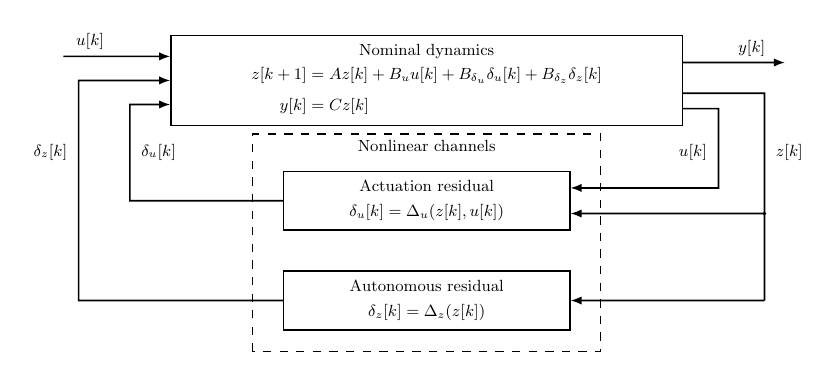
\begin{tikzpicture}[scale=.65,transform shape,x=1cm,y=1cm,block/.style={draw,rectangle,align=center,inner sep=5pt,line width=.6pt,font=\small},wire/.style={line width=.6pt},>={Latex[length=4pt,width=3pt]},every node/.style={font=\small}]
\node[block,minimum width=10cm,minimum height=1.5cm] (nominal) at (0,3.5)
 {Nominal dynamics\\[3pt]
 \mbox{$\begin{aligned}
 z[k+1]&=Az[k]+B_uu[k]+B_{\delta_u}\delta_u[k]+B_{\delta_z}\delta_z[k]\\[3pt]
 y[k]&=Cz[k]
 \end{aligned}$}};
\draw[dashed,line width=.5pt] (-3.4,-1.8) rectangle (3.4,2.45);
\node at (0,2.22) {Nonlinear channels};
\node[block,minimum width=5.6cm,minimum height=1cm] (du) at (0,1.15)
 {Actuation residual\\[3pt] \mbox{$\delta_u[k]=\Delta_u(z[k],u[k])$}};
\node[block,minimum width=5.6cm,minimum height=1cm] (dz) at (0,-.8)
 {Autonomous residual\\[3pt] \mbox{$\delta_z[k]=\Delta_z(z[k])$}};
\draw[wire,->] (-7.1,3.97) -- node[above,pos=.25] {\mbox{$u[k]$}} ([yshift=.47cm]nominal.west);
\draw[wire,->] ([yshift=.35cm]nominal.east) -- (7.0,3.85);
\node[above] at (6.35,3.85) {\mbox{$y[k]$}};
\draw[wire] ([yshift=-.25cm]nominal.east) -- (6.6,3.25) -- (6.6,-.8);

\draw[wire,->] (6.6,.90) -- ([yshift=-.25cm]du.east);
\node[anchor=west] at (6.7,2.1) {\mbox{$z[k]$}};
\draw[wire,->] (6.6,-.8) -- (dz.east);

\fill (6.6,.90) circle[radius=1.1pt];
\draw[wire,->] ([yshift=-.55cm]nominal.east) -- (5.7,2.95) -- (5.7,1.40) -- ([yshift=.25cm]du.east);
\node[anchor=east] at (5.6,2.1) {\mbox{$u[k]$}};
\draw[wire,->] (du.west) -- (-5.8,1.15) -- (-5.8,3.03) -- ([yshift=-.47cm]nominal.west);
\node[anchor=west] at (-5.7,2.1) {\mbox{$\delta_u[k]$}};
\draw[wire,->] (dz.west) -- (-6.8,-.8) -- (-6.8,3.5) -- (nominal.west);
\node[anchor=east] at (-6.9,2.1) {\mbox{$\delta_z[k]$}};
\end{tikzpicture}
\caption{Nominal model with learned nonlinear feedback.
Normalization bounds the residuals relative to the state and applied input.
After reduction, both residuals use the reconstructed state \mbox{$V_r\widehat z$}.}\label{fig:interconnection}
\end{figure}

\subsection{Close the full and reduced feedback loops}
For a projection satisfying Assumption~\ref{ass:reference}, we define the remaining reduced nominal matrices by
\begin{equation}\label{eq:reduced-matrices}
 \widehat A=W_rAV_r,\qquad
 \widehat B_j\eqdef W_rB_j,\qquad
 \widehat C\eqdef CV_r,
 \qquad j\in\{u,\delta_u,\delta_z\}.
\end{equation}
The reduced nonlinear recurrence is
\begin{equation}\label{eq:reduced-channels}
 \widehat z^+=\widehat A\widehat z+\widehat B_uu+
 \widehat B_{\delta_u}\Delta_u(V_r\widehat z,u)+
 \widehat B_{\delta_z}\Delta_z(V_r\widehat z).
\end{equation}
Definition~\ref{def:autonomous-gains} measures how strongly the nominal dynamics amplify injected signals in state coordinates.
The reduction error in \eqref{eq:error}, however, compares outputs, so we next define gains from these same input ports to the observed outputs.

\begin{definition}[Nominal output-channel gains]\label{def:gains}
For each channel \mbox{$j\in\{u,\delta_u,\delta_z\}$}, we define
\begin{equation}\label{eq:gains}
 h_j\eqdef\sup_{w\in\ell_2\setminus\{0\}}
 \frac{\|Cz_j^0\|_{\ell_2}}{\|w\|_{\ell_2}},
 \qquad
 \widehat h_j\eqdef\sup_{w\in\ell_2\setminus\{0\}}
 \frac{\|CV_r\widehat z_j^0\|_{\ell_2}}{\|w\|_{\ell_2}}.
\end{equation}
\end{definition}
We next construct the stability certificate by combining the channel gains above with the residual envelopes in \eqref{eq:reference-split}, enforced by \eqref{eq:neural}.
Because the autonomous residual is driven by the state, we first bound the state response after closing this feedback.
Under the strict margins in Assumption~\ref{ass:reference}, we define
\begin{equation}\label{eq:penalties}
 \begin{aligned}
 \Gamma&\eqdef\frac{g_u+g_{\delta_u}}{1-g_{\delta_z}},&
 \widehat\Gamma&\eqdef
 \frac{\widehat g_u+\widehat g_{\delta_u}}
      {1-\widehat g_{\delta_z}},\\
 \varepsilon&\eqdef h_{\delta_z}\Gamma+h_{\delta_u},&
 \widehat\varepsilon&\eqdef
 \widehat h_{\delta_z}\widehat\Gamma+\widehat h_{\delta_u}.
 \end{aligned}
\end{equation}
For zero initial states, the full and reconstructed reduced states satisfy
\[
 \|z\|_{\ell_2}\le\Gamma\|u\|_{\ell_2},
 \qquad
 \|V_r\widehat z\|_{\ell_2}\le\widehat\Gamma\|u\|_{\ell_2}.
\]
Thus every finite-energy applied input produces finite-energy states in both nonlinear predictors.
Lemma~\ref{lem:departures} in Appendix~\ref{app:feedback} proves these state-gain bounds and the output-departure bounds used below.
It also establishes global exponential stability of both autonomous origin equilibria.

\subsection{Bound the reduction error}
We compare each nonlinear predictor with its nominal response, avoiding a direct bound on the separation of nonlinear trajectories.
The full nominal map \mbox{$\mathcal G^0$} is generated by
\begin{equation}\label{eq:nominal}
 z^0[k+1]=Az^0[k]+B_uu[k],\qquad
 y^0[k]=Cz^0[k],\qquad z^0[0]=0,
\end{equation}
and \mbox{$\widehat{\mathcal G}^0$} uses the reduced nominal matrices.
Since both nominal state matrices are Schur, their difference admits a finite certified gain upper \mbox{$b_r^0$} satisfying
\begin{equation}\label{eq:nominal-error-upper}
 \|\mathcal G^0-\widehat{\mathcal G}^0\|_{\ell_2\to\ell_2}\le b_r^0.
\end{equation}
Appendix~\ref{app:gains} computes such uppers from finite-matrix storage inequalities.

The triangle inequality now separates the comparison into three terms,
\[
 \begin{aligned}
 \mathcal E_r(\theta)
 &\le
 \|\mathcal G_\theta-\mathcal G^0\|_{\ell_2\to\ell_2}
 +\|\mathcal G^0-\widehat{\mathcal G}^0\|_{\ell_2\to\ell_2}\\
 &\qquad+
 \|\widehat{\mathcal G}^0-\widehat{\mathcal G}_\theta\|_{\ell_2\to\ell_2}.
 \end{aligned}
\]
The departure bounds in \eqref{eq:penalties} control the first and third terms.

\begin{definition}[Constructed finite-matrix certificate]\label{def:constructed-certificate}
For the normalized neural family, we include the nominal matrices, physical readout, projection and linear gain witnesses among the parameters.
We evaluate \eqref{eq:penalties} using certified channel-gain uppers consistently in every term and define
\begin{equation}\label{eq:certificate}
 \mathcal B_r(\theta)\eqdef
 \underbrace{\varepsilon}_{\text{full departure}}+
 \underbrace{b_r^0}_{\text{nominal reduction error}}+
 \underbrace{\widehat\varepsilon}_{\text{reduced departure}}.
\end{equation}
This formula applies when the channel and nominal-error witnesses hold, both nominal state matrices are Schur, and both autonomous gain uppers are below one.
We assign \mbox{$+\infty$} otherwise.
\end{definition}

Lemma~\ref{lem:storage-gain} gives finite-matrix storage inequalities that certify the channel gains needed to evaluate this certificate.

\begin{proposition}[Certified nonlinear state reduction]\label{prop:certificate}
The constructed \mbox{$\mathcal B_r$} satisfies Definition~\ref{def:certificate}, with global exponential stability of both autonomous origins.
With matrices and projection fixed, the bound also compares any compatible full and reduced updates satisfying the same global envelopes.
\end{proposition}
\begin{proof}
Lemma~\ref{lem:departures} supplies stability, finite gains and the nonlinear departure bounds.
Combining those bounds with the certified nominal-error upper proves the certificate inequality.
Appendix~\ref{app:certificate} gives the detailed argument.
\end{proof}

Bounding the two nonlinear departures separately makes magnitude envelopes sufficient, but also makes the certificate conservative because it does not exploit cancellation between those departures.
Appendix~\ref{app:lft-comparison} explains why these magnitude envelopes do not directly supply the common-operator error comparison used in LFT reduction.
Corollary~\ref{cor:prescribed-projection} covers the stored projections used in the experiment.

\subsection{Choose a balanced projection}
We specialize to balanced truncation by treating residual ports as independent nominal inputs.

\begin{definition}[Balanced nominal realization]\label{def:balanced}
We define the augmented input matrix by
\[
 B_{\mathrm{aug}}\eqdef[B_u\ B_{\delta_u}\ B_{\delta_z}].
\]
Whenever the Stein solutions
\[
 P=APA^\top+B_{\mathrm{aug}}B_{\mathrm{aug}}^\top,\qquad
 Q=A^\top QA+C^\top C
\]
are positive definite, the classical balancing transformation is an invertible matrix \mbox{$T$} satisfying
\[
 TPT^\top=T^{-\top}QT^{-1}
 =\operatorname{diag}(\sigma_1,\ldots,\sigma_q),
 \qquad \sigma_1\ge\cdots\ge\sigma_q>0.
\]
In balanced coordinates \mbox{$\bar z=Tz$}, we define
\[
 \bar A\eqdef TAT^{-1},\qquad
 \bar B_j\eqdef TB_j,\qquad
 \bar C\eqdef CT^{-1},
 \qquad j\in\{u,\delta_u,\delta_z\}.
\]
For reduced dimension \mbox{$r$}, we define
\[
 \Pi_r\eqdef[I_r\ 0],\qquad
 W_r\eqdef\Pi_rT,\qquad V_r\eqdef T^{-1}\Pi_r^\top.
\]
The reduced nominal matrices in \eqref{eq:reduced-matrices} are then
\[
 \widehat A=\Pi_r\bar A\Pi_r^\top,\qquad
 \widehat B_j=\Pi_r\bar B_j,\qquad
 \widehat C=\bar C\Pi_r^\top.
\]
\end{definition}

When \mbox{$\sigma_r>\sigma_{r+1}$}, balanced truncation gives a Schur reduced nominal matrix and the nominal-error upper
\begin{equation}\label{eq:balanced-nominal-upper}
 b_r^0\eqdef2\sum_{i=r+1}^q\sigma_i
\end{equation}
\citep{antoulas}.
We separately check both feedback margins to certify the resulting nonlinear predictors.

\subsection{Improve fitting without changing the certificate}
Having certified the nonlinear interconnection, we can improve its fit while keeping the reference matrices, projection and gain witnesses fixed.
The normalization that makes this possible also leaves enough freedom to approximate any continuous residual satisfying its prescribed envelope, uniformly on compact sets (Proposition~\ref{prop:density}).
By continuity, sufficiently accurate initialization and updates give accurate full-model predictions over any fixed training horizon.
Increasing neural capacity can therefore drive the full-model fitting loss to zero \emph{under one unchanged certificate}.
This establishes the compatibility of accurate fitting and certified reduction asserted in Theorem~\ref{thm:main}, whose full proof is given in Appendix~\ref{app:joint}.

\section{Example: Accurate prediction and certified reduction}\label{sec:experiments}

We now examine whether the certificate in Theorem~\ref{thm:main} can be applied to reduce a model of a real-world system. A voltage pulse pulls the beam of a micromachined switch toward its substrate, squeezing the air film beneath it \citep{rewienski}.
Predicting this motion requires capturing the coupled beam and pressure dynamics.
We used a physics-based simulation with 96 physical coordinates and learned predictors with eight additional observables, giving 104 states.
We then asked how far these predictors could be reduced while retaining both stability and useful predictions.

We fitted separate predictors with and without residual normalization, training both for full-model and nineteen-state prediction accuracy.
We froze one predictor from each fit before scanning reduction orders or opening the reserved tests, and reduced both by balanced truncation.
The \href{https://github.com/Populustremuloides/certified-nonlinear-reduction}{code repository} and Appendix~\ref{app:experiment} give the training and verification details.

Figure~\ref{fig:central} shows why accurate fitting alone is insufficient.
Both full predictors reproduce the simulated physical response (panel A), and their nineteen-state reductions retain useful prediction accuracy (panel B).
Further reduction, however, exposes a failure absent from the full-model responses.
At nine states, the unnormalized predictor grows explosively, while the normalized predictor returns toward rest (panel C).
The error curves show how prediction performance changes across retained dimensions (panel D).
This instability contrast also appeared on reserved pulses, including cases that tests at smaller amplitudes would have missed.

We verified the small-gain conditions for the normalized full predictor and its nine- and nineteen-state reductions.
These checks give a conservative full-to-reduced error bound and certify global exponential stability and finite input--output gain for every finite-energy applied input.
At nineteen states, useful empirical prediction accuracy therefore accompanies a stability guarantee extending beyond the simulated responses.
The normalized predictor also demonstrates certified reduction beyond the global contraction hypothesis required by \citet{shakib-ren} (Corollary~\ref{cor:figure-contraction-exclusion}).

\begin{figure}[!t]
\centering
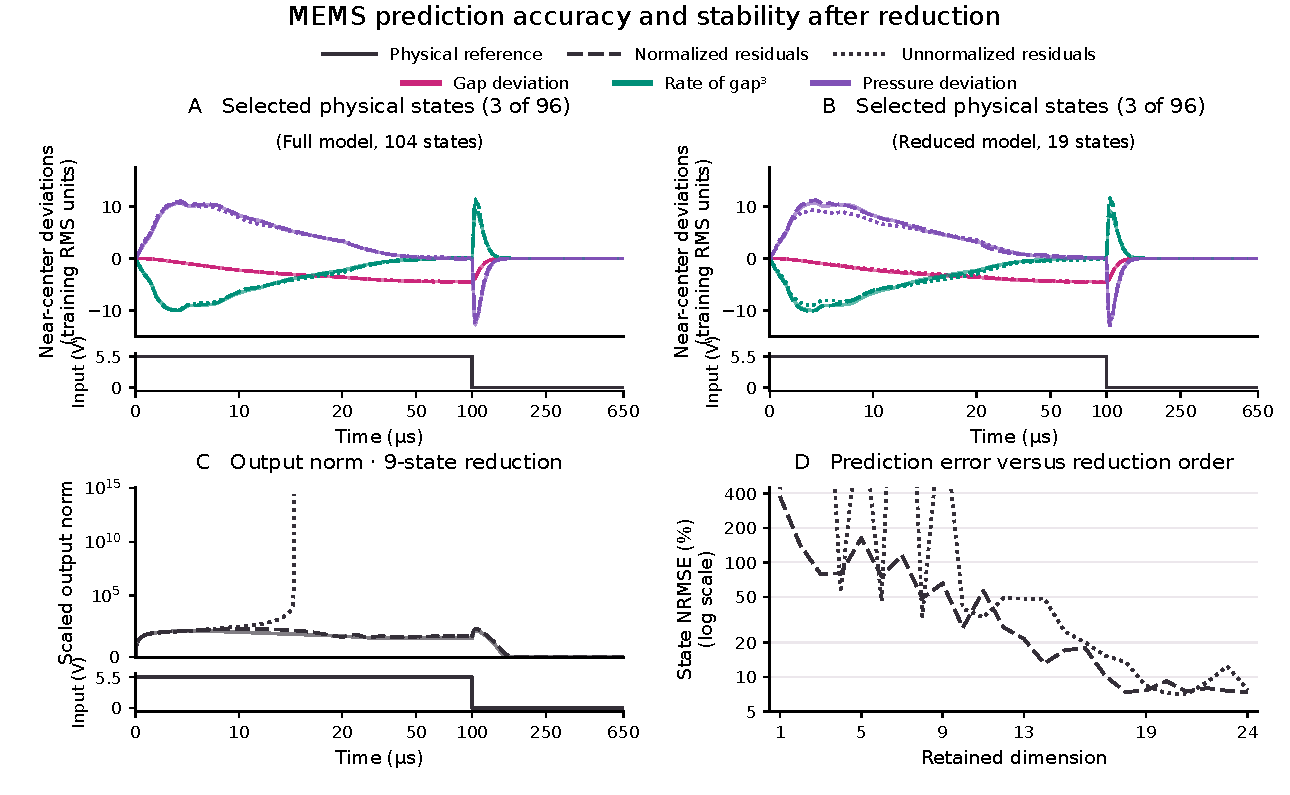
\includegraphics[width=\linewidth,height=0.40\textheight,keepaspectratio]{figures/compact_layout/mems_compact.pdf}
\caption{Empirical prediction accuracy with certified stable reduction.
We fitted two 104-state predictors to a physics-based simulation of a voltage-driven micromachined switch, one with normalized nonlinear residuals and one without, then reduced each by balanced truncation.
(A) Both full predictors track the simulated physical reference.
(B) Their nineteen-state reductions retain prediction accuracy.
(C) At nine states, the unnormalized reduction grows explosively while the normalized reduction returns toward rest.
(D) Error versus retained dimension shows the accuracy cost of further reduction, using one frozen predictor per curve.}\label{fig:central}
\end{figure}


\section{Conclusion}
We learned nonlinear dynamics as corrections to a nominal linear model, normalizing their magnitudes relative to the state and applied input so that finite matrix checks could certify stability before and after reduction (Proposition~\ref{prop:certificate}).
Within the feasible reference class, we proved that fitting could improve to any finite-horizon tolerance while this certificate remained unchanged (Theorem~\ref{thm:main}).
Our micromachined-switch example demonstrated the practical value of this construction, combining useful reduced prediction accuracy with certified stability beyond the global contraction hypothesis required by \citet{shakib-ren} (Corollary~\ref{cor:figure-contraction-exclusion}).

\label{main-text-end}

\subsection*{Generative AI Use}
We used generative AI tools, including ChatGPT/Codex and Claude, to assist with research development, literature review, mathematical arguments, experimental implementation, Lean formalization, and manuscript drafting and editing.
The authors remain responsible for the accuracy and integrity of the submitted work.

\clearpage
\begin{thebibliography}{99}
\bibitem[Abbasi et~al.(2022)]{abbasi}
M. H. Abbasi, L. Iapichino, W. Schilders, and N. van de Wouw.
\newblock A data-based stability-preserving model order reduction method for hyperbolic partial differential equations.
\newblock \emph{Nonlinear Dynamics}, 107:3729--3748, 2022.
\newblock doi:10.1007/s11071-021-07094-8.

\bibitem[Antoulas(2005)]{antoulas}
A. C. Antoulas.
\newblock \emph{Approximation of Large-Scale Dynamical Systems}.
\newblock SIAM, 2005. doi:10.1137/1.9780898718713.

\bibitem[Beck et~al.(1996)]{beck-lft}
C. L. Beck, J. Doyle, and K. Glover.
\newblock Model reduction of multidimensional and uncertain systems.
\newblock \emph{IEEE Transactions on Automatic Control}, 41(10):1466--1477, 1996.
\newblock doi:10.1109/9.539427.

\bibitem[Besselink et~al.(2013)]{besselink-feedback}
B. Besselink, N. van de Wouw, and H. Nijmeijer.
\newblock Model reduction for nonlinear systems with incremental gain or passivity properties.
\newblock \emph{Automatica}, 49(4):861--872, 2013.
\newblock doi:10.1016/j.automatica.2013.01.004.

\bibitem[Besselink et~al.(2014)]{besselink-incremental}
B. Besselink, N. van de Wouw, J. M. A. Scherpen, and H. Nijmeijer.
\newblock Model reduction for nonlinear systems by incremental balanced truncation.
\newblock \emph{IEEE Transactions on Automatic Control}, 59(10):2739--2753, 2014.
\newblock doi:10.1109/TAC.2014.2326548.

\bibitem[Bond and Daniel(2009)]{bond-daniel}
B. N. Bond and L. Daniel.
\newblock Stable reduced models for nonlinear descriptor systems through piecewise-linear approximation and projection.
\newblock \emph{IEEE Transactions on Computer-Aided Design of Integrated Circuits and Systems}, 28(10):1467--1480, 2009.
\newblock doi:10.1109/TCAD.2009.2030596.

\bibitem[Brown and King(2025)]{brown-gramians}
B. C. Brown and M. King.
\newblock Gramians for a new class of nonlinear control systems using Koopman and a novel generalized SVD.
\newblock arXiv:2507.04188v2, 2025.
\bibitem[Forgione et~al.(2024)]{forgione}
M. Forgione, M. Mejari, and D. Piga.
\newblock Model order reduction of deep structured state-space models. A system-theoretic approach.
\newblock arXiv:2403.14833, 2024.

\bibitem[Fujimoto and Scherpen(2005)]{fujimoto}
K. Fujimoto and J. M. A. Scherpen.
\newblock Nonlinear input-normal realizations based on the differential eigenstructure of Hankel operators.
\newblock \emph{IEEE Transactions on Automatic Control}, 50(1):2--18, 2005.

\bibitem[Haseli and Cort\'es(2025)]{haseli}
M. Haseli and J. Cort\'es.
\newblock Modeling nonlinear control systems via Koopman control family. Universal forms and subspace invariance proximity.
\newblock arXiv:2307.15368v4, 2025.

\bibitem[Kawano(2021)]{kawano}
Y. Kawano.
\newblock Controller reduction for nonlinear systems by generalized differential balancing.
\newblock arXiv:2111.03209, 2021.

\bibitem[Kawano and Scherpen(2017)]{kawano-scherpen}
Y. Kawano and J. M. A. Scherpen.
\newblock Model reduction by differential balancing based on nonlinear Hankel operators.
\newblock \emph{IEEE Transactions on Automatic Control}, 62(7):3293--3308, 2017.

\bibitem[Koopman(1931)]{koopman}
B. O. Koopman.
\newblock Hamiltonian systems and transformation in Hilbert space.
\newblock \emph{Proceedings of the National Academy of Sciences}, 17(5):315--318, 1931.
\newblock doi:10.1073/pnas.17.5.315.

\bibitem[Korda and Mezi\'c(2018)]{korda-mezic}
M. Korda and I. Mezi\'c.
\newblock Linear predictors for nonlinear dynamical systems. Koopman operator meets model predictive control.
\newblock \emph{Automatica}, 93:149--160, 2018.
\newblock doi:10.1016/j.automatica.2018.03.046.

\bibitem[Lall and Beck(1999)]{lall-beck-lft}
S. Lall and C. Beck.
\newblock Model reduction of complex systems in the linear-fractional framework.
\newblock In \emph{Proceedings of the IEEE International Symposium on Computer Aided Control System Design}, pages 34--39, 1999.
\newblock doi:10.1109/CACSD.1999.808620.

\bibitem[Leshno et~al.(1993)]{leshno}
M. Leshno, V. Y. Lin, A. Pinkus, and S. Schocken.
\newblock Multilayer feedforward networks with a nonpolynomial activation function can approximate any function.
\newblock \emph{Neural Networks}, 6(6):861--867, 1993.
\newblock doi:10.1016/S0893-6080(05)80131-5.

\bibitem[Lusch et~al.(2018)]{lusch}
B. Lusch, J. N. Kutz, and S. L. Brunton.
\newblock Deep learning for universal linear embeddings of nonlinear dynamics.
\newblock \emph{Nature Communications}, 9:4950, 2018.
\newblock doi:10.1038/s41467-018-07210-0.

\bibitem[Manek and Kolter(2019)]{manek-kolter}
G. Manek and J. Z. Kolter.
\newblock Learning stable deep dynamics models.
\newblock In \emph{Advances in Neural Information Processing Systems}, volume 32, 2019.

\bibitem[Mezi\'c(2005)]{mezic}
I. Mezi\'c.
\newblock Spectral properties of dynamical systems, model reduction and decompositions.
\newblock \emph{Nonlinear Dynamics}, 41:309--325, 2005.
\newblock doi:10.1007/s11071-005-2824-x.

\bibitem[Pulch(2019)]{pulch-projection}
R. Pulch.
\newblock Stability preservation in Galerkin-type projection-based model order reduction.
\newblock \emph{Numerical Algebra, Control and Optimization}, 9(1):23--44, 2019.
\newblock doi:10.3934/naco.2019003.

\bibitem[Revay et~al.(2021)]{ren}
M. Revay, R. Wang, and I. R. Manchester.
\newblock Recurrent equilibrium networks. Flexible dynamic models with guaranteed stability and robustness.
\newblock arXiv:2104.05942, 2021.

\bibitem[Rewienski(2003)]{rewienski}
M. Rewienski.
\newblock \emph{A Trajectory Piecewise-Linear Approach to Model Order Reduction of Nonlinear Dynamical Systems}.
\newblock PhD thesis, Massachusetts Institute of Technology, 2003.
\bibitem[Scherpen(1993)]{scherpen}
J. M. A. Scherpen.
\newblock Balancing for nonlinear systems.
\newblock \emph{Systems \& Control Letters}, 21(2):143--153, 1993.
\newblock doi:10.1016/0167-6911(93)90117-O.

\bibitem[Shakib(2025)]{shakib-ren}
M. F. Shakib.
\newblock State dimension reduction of recurrent equilibrium networks with contraction and robustness preservation.
\newblock arXiv:2508.02843, 2025.

\bibitem[Vasilyev et~al.(2003)]{vasilyev-dac}
D. Vasilyev, M. Rewienski, and J. White.
\newblock A TBR-based trajectory piecewise-linear algorithm for generating accurate low-order models for nonlinear analog circuits and MEMS.
\newblock In \emph{Proceedings of the 40th Design Automation Conference}, pages 490--495, 2003.

\bibitem[Williams et~al.(2015)]{williams-edmd}
M. O. Williams, I. G. Kevrekidis, and C. W. Rowley.
\newblock A data-driven approximation of the Koopman operator. Extending dynamic mode decomposition.
\newblock \emph{Journal of Nonlinear Science}, 25(6):1307--1346, 2015.
\newblock doi:10.1007/s00332-015-9258-5.

\bibitem[Yeung et~al.(2018)]{yeung}
E. Yeung, Z. Liu, and N. O. Hodas.
\newblock A Koopman operator approach for computing and balancing Gramians for discrete time nonlinear systems.
\newblock In \emph{Proceedings of the American Control Conference}, pages 337--344, 2018.
\newblock doi:10.23919/ACC.2018.8431738.

\end{thebibliography}
\clearpage
\appendix
\section{Prescribed-envelope neural approximation}\label{app:approximation}
This appendix proves the approximation used in Theorem~\ref{thm:main}.
The injection matrices are fixed throughout.
In particular, approximation does not enlarge an autonomous feedback gain.

For a fixed full-row-rank physical readout and a finite ReLU lifting network \mbox{$\psi_\theta:\R^n\to\R^q$}, we define
\begin{equation}\label{eq:lifting}
 \begin{gathered}
 C_x^\dagger\eqdef C_x^\top(C_xC_x^\top)^{-1},\\
 \Phi_\theta(x)\eqdef C_x^\dagger x+
 (I_q-C_x^\dagger C_x)[\psi_\theta(x)-\psi_\theta(0)].
 \end{gathered}
\end{equation}
This preserves \mbox{$C_x\Phi_\theta(x)=x$} and \mbox{$\Phi_\theta(0)=0$} while allowing finite neural approximation of the added observables.

\begin{proposition}[Approximation within prescribed envelopes]\label{prop:density}\leavevmode\par
For continuous residual factors obeying \eqref{eq:reference-split} on nonempty compact sets \mbox{$\mathcal K_z\subset\R^q$} and \mbox{$\mathcal K_u\subset\R^m$},
\[
 \inf_{a_\theta,c_\theta}
 \max\left\{
 \sup_{\mathcal K_z}\|\Delta_z^*-\Delta_{z,\theta}\|_2,\
 \sup_{\mathcal K_z\times\mathcal K_u}\|\Delta_u^*-\Delta_{u,\theta}\|_2
 \right\}=0.
\]
The infimum ranges over finite networks of unrestricted capacity.
The injection matrices remain fixed.
\end{proposition}
% Lean correspondence prop:density -> Populus.ModelReduction.Certified.approximation_within_prescribed_envelopes
\leanref{Proposition~\ref{prop:density}}{Populus/Chapters/NonlinearModelReductionWithErrorBounds/CertifiedReduction/ResidualApproximation.lean}{approximation_within_prescribed_envelopes}


For \mbox{$p\in\mathbb N$}, we define the radial projection
\[
 \operatorname{rad}_p(v)\eqdef\frac{v}{\max\{1,\|v\|_2\}},\qquad v\in\R^p.
\]
It is the Euclidean projection onto the closed unit ball and is nonexpansive.
Let \mbox{$\mathcal K\subset\R^b$} be nonempty and compact, let \mbox{$\rho:\R^b\to[0,\infty)$} be continuous, and let \mbox{$e:\mathcal K\to\R^p$} be continuous with
\[
 \|e(v)\|_2\le\rho(v),\qquad e_\theta(v)\eqdef\rho(v)\operatorname{rad}_p(h_\theta(v)).
\]
Here \mbox{$h_\theta:\R^b\to\R^p$} is a finite ReLU coefficient network.

\begin{lemma}[Uniform approximation with a fixed driving envelope]\label{lem:fixed-envelope}
For every \mbox{$\epsilon>0$}, there is a finite network \mbox{$h_\theta$} such that
\[
 \sup_{v\in\mathcal K}\|e(v)-e_\theta(v)\|_2<\epsilon.
\]
For every parameter choice, \mbox{$\|e_\theta(v)\|_2\le\rho(v)$} for all \mbox{$v\in\R^b$}.
\end{lemma}
% Lean correspondence lem:fixed-envelope -> Populus.ModelReduction.Certified.uniform_approximation_with_fixed_driving_envelope
\leanref{Lemma~\ref{lem:fixed-envelope}}{Populus/Chapters/NonlinearModelReductionWithErrorBounds/CertifiedReduction/EnvelopeApproximation.lean}{uniform_approximation_with_fixed_driving_envelope}

\begin{proof}
Fix \mbox{$\epsilon>0$} and define, for \mbox{$\eta>0$},
\[
 d_\eta(v)\eqdef\frac{e(v)}{\max\{\rho(v),\eta\}},\qquad
 \rho_{\max}\eqdef\max_{v\in\mathcal K}\rho(v).
\]
Then
\[
 \begin{aligned}
 \max\{\rho(v),\eta\}&\ge\eta>0
 &&\text{(positive denominator)},\\
 \|d_\eta(v)\|_2
 &\le\frac{\rho(v)}{\max\{\rho(v),\eta\}}\le1
 &&\text{(prescribed envelope)},\\
 \operatorname{rad}_p(d_\eta(v))&=d_\eta(v)
 &&\text{(unit-ball projection)}.
 \end{aligned}
\]
Continuity on \mbox{$\mathcal K$} and universal approximation \citep{leshno} give a finite ReLU network with
\[
 \sup_{\mathcal K}\|h_\theta-d_\eta\|_2<\delta.
\]
Consequently,
\[
 \begin{aligned}
 \|\operatorname{rad}_p(h_\theta(v))-d_\eta(v)\|_2
 &\le\|h_\theta(v)-d_\eta(v)\|_2
 &&\text{(nonexpansiveness)},\\
 \|e(v)-\rho(v)d_\eta(v)\|_2
 &=\begin{cases}
 0,&\rho(v)\ge\eta,\\
 (1-\rho(v)/\eta)\|e(v)\|_2,&\rho(v)<\eta
 \end{cases}\\
 &\le\eta
 &&\text{(prescribed envelope)},\\
 \|e(v)-e_\theta(v)\|_2
 &\le\|e(v)-\rho(v)d_\eta(v)\|_2\\
 &\quad+\rho(v)\|d_\eta(v)-\operatorname{rad}_p(h_\theta(v))\|_2
 &&\text{(triangle inequality)}.
 \end{aligned}
\]
Choose \mbox{$0<\eta<\epsilon/2$} and \mbox{$0<\delta<\epsilon/[2(1+\rho_{\max})]$} to obtain
\[
 \sup_{\mathcal K}\|e-e_\theta\|_2
 \le\eta+\rho_{\max}\delta<\epsilon.
\]
For every parameter choice and every \mbox{$v\in\R^b$},
\[
 \|e_\theta(v)\|_2
 =\rho(v)\|\operatorname{rad}_p(h_\theta(v))\|_2
 \le\rho(v).
\]
\end{proof}
\begin{proof} of Proposition~\ref{prop:density}.
Apply Lemma~\ref{lem:fixed-envelope} to the two channels with
\[
 \begin{array}{c|c|c|c}
 &v&\rho(v)&e(v)\\\hline
 \text{autonomous}&z&\|z\|_2&\Delta_z^*(z)\\
 \text{actuation}&(z,u)&\|u\|_2&\Delta_u^*(z,u).
 \end{array}
\]
For every \mbox{$\epsilon>0$}, the resulting finite networks satisfy
\[
 \max\left\{
 \sup_{\mathcal K_z}\|\Delta_z^*-\Delta_{z,\theta}\|_2,
 \sup_{\mathcal K_z\times\mathcal K_u}\|\Delta_u^*-\Delta_{u,\theta}\|_2
 \right\}<\epsilon.
\]
For any fixed injection \mbox{$B_\delta$},
\[
 \sup_{\mathcal K}\|B_\delta(e-e_\theta)\|_2
 \le\|B_\delta\|_{2\to2}\sup_{\mathcal K}\|e-e_\theta\|_2
 \longrightarrow0,
\]
without a rank condition on \mbox{$B_\delta$}.
\end{proof}

\subsection{A norm-preserving reservoir implementation}
A smooth normalization with an identity reservoir gives the implementation used in the matched protocol.
Let \mbox{$w:\R^b\to\R^d$} be a continuous driving map and \mbox{$h_\theta:\R^b\to\R^p$} a finite coefficient network.
Define
\begin{equation}\label{eq:reservoir}
 \Omega_\theta(v)\eqdef
 \frac{1}{\sqrt{1+\|h_\theta(v)\|_2^2}}
 \begin{bmatrix}\|w(v)\|_2h_\theta(v)\\w(v)\end{bmatrix},
 \qquad \|\Omega_\theta(v)\|_2=\|w(v)\|_2.
\end{equation}
The norm-preservation identity in \eqref{eq:reservoir} follows by squaring the norm.
For autonomy, \mbox{$v=z$} and \mbox{$w(v)=z$}.
For actuation, \mbox{$v=(z,u)$} and \mbox{$w(v)=u$}.

\begin{proposition}[Prescribed-envelope reservoir density]\label{prop:reservoir}
Use the driving norm \mbox{$\rho(v)=\|w(v)\|_2$} in Lemma~\ref{lem:fixed-envelope}.
For a fixed injection \mbox{$B_\delta$}, residuals of the form
\[
 [B_\delta\ 0]\Omega_\theta(v)
\]
approximate \mbox{$B_\delta e(v)$} uniformly on \mbox{$\mathcal K$}.
The extended injection has the same Gramian product and linear induced gains as \mbox{$B_\delta$}.
\end{proposition}
% Lean correspondence prop:reservoir -> Populus.ModelReduction.Certified.prescribed_envelope_reservoir_density
\leanref{Proposition~\ref{prop:reservoir}}{Populus/Chapters/NonlinearModelReductionWithErrorBounds/CertifiedReduction/ReservoirDensity.lean}{prescribed_envelope_reservoir_density}

\begin{proof}
First, the reservoir preserves the driving norm,
\[
 \|\Omega_\theta(v)\|_2^2
 =\frac{\|w(v)\|_2^2\|h_\theta(v)\|_2^2+\|w(v)\|_2^2}
        {1+\|h_\theta(v)\|_2^2}
 =\|w(v)\|_2^2.
\]
Fix \mbox{$0<\eta<1$} and define
\[
 \begin{gathered}
 \rho_{\max}\eqdef\max_{\mathcal K}\rho,\qquad
 d_\eta(v)\eqdef(1-\eta)\frac{e(v)}{\max\{\rho(v),\eta\}},\\
 h_\eta(v)\eqdef\frac{d_\eta(v)}{\sqrt{1-\|d_\eta(v)\|_2^2}},\qquad
 \nu(h)\eqdef\frac{h}{\sqrt{1+\|h\|_2^2}}.
 \end{gathered}
\]
The continuous maps \mbox{$d_\eta,h_\eta$} satisfy
\[
 \begin{aligned}
 \|d_\eta(v)\|_2&\le1-\eta<1
 &&\text{(prescribed envelope)},\\
 1+\|h_\eta(v)\|_2^2
 &=\frac{1}{1-\|d_\eta(v)\|_2^2},\\
 \nu(h_\eta(v))&=d_\eta(v)
 &&\text{(substitution)},\\
 \|e(v)-\rho(v)d_\eta(v)\|_2
 &\le\begin{cases}
 \eta\rho_{\max},&\rho(v)\ge\eta,\\
 \eta,&\rho(v)<\eta
 \end{cases}\\
 &\le\eta(1+\rho_{\max}).
 \end{aligned}
\]
The normalization map is nonexpansive because
\[
 \begin{aligned}
 D\nu(h)
 &=\frac{I}{\sqrt{1+\|h\|_2^2}}
   -\frac{hh^\top}{(1+\|h\|_2^2)^{3/2}},\\
 \|D\nu(h)\|_{2\to2}&\le1
 &&\text{(radial and tangential eigenvalues)},\\
 \|\nu(h)-\nu(\widetilde h)\|_2&\le\|h-\widetilde h\|_2
 &&\text{(integration along the segment)}.
 \end{aligned}
\]
A finite network with \mbox{$\sup_{\mathcal K}\|h_\theta-h_\eta\|_2<\delta$} therefore gives
\[
 \begin{aligned}
 {}[B_\delta\ 0]\Omega_\theta(v)
 &=B_\delta\rho(v)\nu(h_\theta(v)),\\
 \sup_{\mathcal K}\|B_\delta e-[B_\delta\ 0]\Omega_\theta\|_2
 &\le\|B_\delta\|_{2\to2}
 \left[\eta(1+\rho_{\max})+\rho_{\max}\delta\right]
 &&\text{(triangle inequality)}\\
 &\longrightarrow0
 &&\text{as }\eta,\delta\downarrow0.
 \end{aligned}
\]
Let \mbox{$\mathcal T_B$} denote any zero-state nominal channel with injection \mbox{$B$} and a fixed state or output observation.
Then
\[
 \begin{aligned}
 {}[B_\delta\ 0][B_\delta\ 0]^\top&=B_\delta B_\delta^\top,\\
 \mathcal T_{[B_\delta\ 0]}(w_1,w_2)&=\mathcal T_{B_\delta}(w_1),\\
 \|\mathcal T_{[B_\delta\ 0]}\|_{\ell_2\to\ell_2}
 &\le\|\mathcal T_{B_\delta}\|_{\ell_2\to\ell_2}
 &&\text{since }\|w_1\|_{\ell_2}\le\|(w_1,w_2)\|_{\ell_2},\\
 \|\mathcal T_{[B_\delta\ 0]}\|_{\ell_2\to\ell_2}
 &\ge\|\mathcal T_{B_\delta}\|_{\ell_2\to\ell_2}
 &&\text{by restricting to }w_2=0.\quad\BlackBox
 \end{aligned}
\]
\renewcommand*{\jmlrQED}{\par\bigskip}
\end{proof}

\section{Linear channel-gain certificates}\label{app:gains}
All nonlinear bounds in the paper reduce to gains of finite-dimensional linear systems.
We use storage witnesses to certify these gains from finite matrices.

\subsection{Bounded-real storage witnesses}
Fix dimensions \mbox{$d_g,b_g,c_g\in\mathbb N$}, matrices \mbox{$A_g\in\R^{d_g\times d_g}$}, \mbox{$B_g\in\R^{d_g\times b_g}$}, \mbox{$C_g\in\R^{c_g\times d_g}$}, and the zero-state response \mbox{$s[k+1]=A_gs[k]+B_gw[k]$}, \mbox{$s[0]=0$}.
\begin{lemma}[Certified linear channel gain]\label{lem:storage-gain}
Suppose \mbox{$A_g$} is Schur, \mbox{$X_g\in\R^{d_g\times d_g}$} is symmetric positive definite, and \mbox{$g\ge0$} satisfies
\begin{equation}\label{eq:brl}
 \begin{bmatrix}
 A_g^\top X_g A_g-X_g+C_g^\top C_g&A_g^\top X_g B_g\\
 B_g^\top X_g A_g&B_g^\top X_g B_g-g^2I
 \end{bmatrix}\preceq0.
\end{equation}
Then
\[
 \|C_gs\|_{\ell_2}\le g\|w\|_{\ell_2}\qquad\forall w\in\ell_2.
\]
For every \mbox{$g$} strictly greater than the true channel gain, a positive-definite strict storage witness exists.
\end{lemma}
% Lean correspondence lem:storage-gain -> Populus.ModelReduction.Certified.certified_linear_channel_gain
\leanref{Lemma~\ref{lem:storage-gain}}{Populus/Chapters/NonlinearModelReductionWithErrorBounds/CertifiedReduction/StrictBoundedReal.lean}{certified_linear_channel_gain}

\begin{proof}
Define \mbox{$V_g(s)\eqdef s^\top X_gs\ge0$} and let \mbox{$\mathscr Q_g$} denote the matrix in \eqref{eq:brl}.
Along the recurrence,
\[
 s[k+1]=A_gs[k]+B_gw[k],
\]
we have
\[
 \begin{aligned}
 &V_g(s[k+1])-V_g(s[k])
   +\|C_gs[k]\|_2^2-g^2\|w[k]\|_2^2\\
 &\qquad=\begin{bmatrix}s[k]\\w[k]\end{bmatrix}^{\!\top}
 \mathscr Q_g\begin{bmatrix}s[k]\\w[k]\end{bmatrix}
 \le0
 \qquad\text{by \eqref{eq:brl}}.
 \end{aligned}
\]
Summing from \mbox{$k=0$} to \mbox{$K$} gives
\[
 \begin{aligned}
 V_g(s[K+1])-V_g(s[0])
 +\sum_{k=0}^K\|C_gs[k]\|_2^2
 &\le g^2\sum_{k=0}^K\|w[k]\|_2^2
 &&\text{(telescoping)},\\
 \|C_gs\|_{\ell_2[0,K]}^2
 &\le g^2\|w\|_{\ell_2[0,K]}^2-V_g(s[K+1])
 &&\text{since }s[0]=0,\\
 &\le g^2\|w\|_{\ell_2[0,K]}^2
 &&\text{since }X_g\succ0.
 \end{aligned}
\]
Thus
\[
 \|C_gs\|_{\ell_2}^2
 =\lim_{K\to\infty}\|C_gs\|_{\ell_2[0,K]}^2
 \le g^2\|w\|_{\ell_2}^2
 \qquad\text{(monotone limits)}.
\]
The strict witness assertion follows from the bounded-real lemma for Schur \mbox{$A_g$} \citep{antoulas}.
\end{proof}
Finite-matrix searches therefore permit arbitrarily close gain uppers when a strict feedback margin requires them.

\subsection{Nominal physical-input error}
For any feasible projection, define the nominal error realization by
\[
 A_e\eqdef\operatorname{diag}(A,\widehat A),\qquad
 B_e\eqdef\begin{bmatrix}B_u\\\widehat B_u\end{bmatrix},\qquad
 C_e\eqdef[C\ -\widehat C].
\]
Applying Lemma~\ref{lem:storage-gain} to this realization gives a finite certified upper \mbox{$b_r^0$} on the nominal physical-input error.
For balanced truncation, the Hankel-tail upper in \eqref{eq:balanced-nominal-upper} is also valid \citep{antoulas}.
If \mbox{$B_u=0$}, both nominal physical-input responses vanish and \mbox{$b_r^0=0$} is valid.

\section{Finite-horizon feedback estimates and stability of the origin equilibria}\label{app:feedback}
\begin{lemma}[Nonlinear departures and stability]\label{lem:departures}
Suppose \mbox{$A,\widehat A$} are Schur, both global residual envelopes hold, and \mbox{$g_{\delta_z},\widehat g_{\delta_z}<1$}.
For zero initial states,
\[
 \|z\|_{\ell_2}\le\Gamma\|u\|_{\ell_2},\qquad
 \|V_r\widehat z\|_{\ell_2}\le\widehat\Gamma\|u\|_{\ell_2},
\]
\[
 \|\mathcal G-\mathcal G^0\|_{\ell_2\to\ell_2}\le\varepsilon,
 \qquad
 \|\widehat{\mathcal G}-\widehat{\mathcal G}^0\|_{\ell_2\to\ell_2}\le\widehat\varepsilon.
\]
Both autonomous origin equilibria are globally exponentially stable, and both zero-state input--output gains are finite.
\end{lemma}
% Lean correspondence lem:departures -> Populus.ModelReduction.Certified.nonlinear_departures_and_stability
\leanref{Lemma~\ref{lem:departures}}{Populus/Chapters/NonlinearModelReductionWithErrorBounds/CertifiedReduction/DeparturesLemma.lean}{nonlinear_departures_and_stability}

We prove Lemma~\ref{lem:departures} on finite prefixes before taking infinite-horizon limits.
This avoids assuming finite state energy in the estimate that is meant to prove it.

\begin{proof} of Lemma~\ref{lem:departures}.
\subsection{Full-model energy and departure}
For \mbox{$K\in\mathbb N_0$}, define
\[
 \begin{gathered}
 \delta_u[k]\eqdef\Delta_u(z[k],u[k]),\qquad
 \delta_z[k]\eqdef\Delta_z(z[k]),\\
 Z_K\eqdef\|z\|_{\ell_2[0,K]},\qquad
 U_K\eqdef\|u\|_{\ell_2[0,K]}.
 \end{gathered}
\]
Causality makes the response to an input truncated after \mbox{$K$} agree with the original response through \mbox{$K$}.
The zero-state channel gains therefore give
\[
 \begin{aligned}
 Z_K
 &\le g_uU_K+g_{\delta_u}\|\delta_u\|_{\ell_2[0,K]}
            +g_{\delta_z}\|\delta_z\|_{\ell_2[0,K]}
 &&\text{(superposition and channel gains)}\\
 &\le(g_u+g_{\delta_u})U_K+g_{\delta_z}Z_K
 &&\text{(residual envelopes)},\\
 (1-g_{\delta_z})Z_K&\le(g_u+g_{\delta_u})U_K,\\
 Z_K&\le\frac{g_u+g_{\delta_u}}{1-g_{\delta_z}}U_K=\Gamma U_K
 &&\text{since }g_{\delta_z}<1,\\
 \|z\|_{\ell_2}&=\lim_{K\to\infty}Z_K\le\Gamma\|u\|_{\ell_2}
 &&\text{(monotone limits)}.
 \end{aligned}
\]
Both nominal and nonlinear responses start at zero, so
\[
 \begin{aligned}
 \|y-y^0\|_{\ell_2}
 &\le h_{\delta_u}\|\delta_u\|_{\ell_2}
      +h_{\delta_z}\|\delta_z\|_{\ell_2}
 &&\text{(output-channel gains)}\\
 &\le(h_{\delta_u}+h_{\delta_z}\Gamma)\|u\|_{\ell_2}
 &&\text{(envelopes and state bound)}\\
 &=\varepsilon\|u\|_{\ell_2},\\
 \|y\|_{\ell_2}
 &\le\|y^0\|_{\ell_2}+\|y-y^0\|_{\ell_2}
 &&\text{(triangle inequality)}\\
 &\le(h_u+\varepsilon)\|u\|_{\ell_2}<\infty.
 \end{aligned}
\]
\subsection{Reduced-model energy measured on its reconstruction}
Define
\[
 \begin{gathered}
 \eta[k]\eqdef V_r\widehat z[k],\qquad
 \widehat Z_K\eqdef\|\eta\|_{\ell_2[0,K]},\\
 \widehat\delta_u[k]\eqdef\Delta_u(\eta[k],u[k]),\qquad
 \widehat\delta_z[k]\eqdef\Delta_z(\eta[k]).
 \end{gathered}
\]
Using the reconstructed-state observation \mbox{$V_r$} in the channel gains,
\[
 \begin{aligned}
 \widehat Z_K
 &\le\widehat g_uU_K
   +\widehat g_{\delta_u}\|\widehat\delta_u\|_{\ell_2[0,K]}
   +\widehat g_{\delta_z}\|\widehat\delta_z\|_{\ell_2[0,K]}\\
 &\le(\widehat g_u+\widehat g_{\delta_u})U_K
       +\widehat g_{\delta_z}\widehat Z_K
 &&\text{(residual envelopes)},\\
 (1-\widehat g_{\delta_z})\widehat Z_K
 &\le(\widehat g_u+\widehat g_{\delta_u})U_K,\\
 \widehat Z_K&\le\widehat\Gamma U_K
 &&\text{since }\widehat g_{\delta_z}<1,\\
 \|V_r\widehat z\|_{\ell_2}
 &=\lim_{K\to\infty}\widehat Z_K
 \le\widehat\Gamma\|u\|_{\ell_2}.
 \end{aligned}
\]
The output estimates follow in the same coordinates,
\[
 \begin{aligned}
 \|\widehat y-\widehat y^0\|_{\ell_2}
 &\le\widehat h_{\delta_u}\|\widehat\delta_u\|_{\ell_2}
    +\widehat h_{\delta_z}\|\widehat\delta_z\|_{\ell_2}
 &&\text{(output-channel gains)}\\
 &\le(\widehat h_{\delta_u}
       +\widehat h_{\delta_z}\widehat\Gamma)\|u\|_{\ell_2}
 &&\text{(envelopes and state bound)}\\
 &=\widehat\varepsilon\|u\|_{\ell_2},\\
 \|\widehat y\|_{\ell_2}
 &\le\|\widehat y^0\|_{\ell_2}
      +\|\widehat y-\widehat y^0\|_{\ell_2}\\
 &\le(\widehat h_u+\widehat\varepsilon)\|u\|_{\ell_2}<\infty.
 \end{aligned}
\]
\subsection{Global exponential stability of the origin equilibria}
At zero input, the envelopes imply
\[
 \Delta_z(0)=0,\qquad\Delta_u(z,0)=0,\qquad
 \widetilde F(0,0)=0,\qquad W_r\widetilde F(V_r0,0)=0.
\]
Schur stability supplies the finite constants
\[
 c\eqdef\left(\sum_{k=0}^\infty\|A^k\|_{2\to2}^2\right)^{1/2},\qquad
 \widehat c\eqdef
 \left(\sum_{k=0}^\infty\|V_r\widehat A^k\|_{2\to2}^2\right)^{1/2}.
\]
Including the free response in each prefix estimate gives
\[
 \begin{aligned}
 Z_K&\le c\|z[0]\|_2+g_{\delta_z}Z_K,\\
 Z_K&\le\frac{c}{1-g_{\delta_z}}\|z[0]\|_2
 &&\text{(strict full margin)},\\
 \widehat Z_K&\le\widehat c\|\widehat z[0]\|_2
                    +\widehat g_{\delta_z}\widehat Z_K,\\
 \widehat Z_K&\le\frac{\widehat c}{1-\widehat g_{\delta_z}}
                         \|\widehat z[0]\|_2
 &&\text{(strict reduced margin)},\\
 \|\widehat z[k]\|_2
 &=\|W_rV_r\widehat z[k]\|_2
 \le\|W_r\|_{2\to2}\|\eta[k]\|_2
 &&\text{since }W_rV_r=I_r.
 \end{aligned}
\]
With
\[
 M_0\eqdef\frac{c^2}{(1-g_{\delta_z})^2}\ge1,\qquad
 \widehat M_0\eqdef\max\left\{1,
 \frac{\|W_r\|_{2\to2}^2\widehat c^2}
      {(1-\widehat g_{\delta_z})^2}\right\},
\]
taking monotone limits yields
\begin{equation}\label{eq:summed-energy}
 \sum_{k=0}^\infty\|z[k]\|_2^2\le M_0\|z[0]\|_2^2,
 \qquad
 \sum_{k=0}^\infty\|\widehat z[k]\|_2^2
 \le\widehat M_0\|\widehat z[0]\|_2^2.
\end{equation}
For either autonomous update \mbox{$f:\R^d\to\R^d$}, let \mbox{$\xi[k;\xi_0]$} denote its trajectory and let \mbox{$M$} be its constant in \eqref{eq:summed-energy}.
Define
\[
 \Upsilon(\xi)\eqdef\sum_{k=0}^\infty\|\xi[k;\xi]\|_2^2.
\]
Then
\[
 \begin{aligned}
 \|\xi\|_2^2&\le\Upsilon(\xi)\le M\|\xi\|_2^2
 &&\text{by \eqref{eq:summed-energy}},\\
 \Upsilon(f(\xi))
 &=\Upsilon(\xi)-\|\xi\|_2^2
 &&\text{(shift the trajectory sum)}\\
 &\le(1-M^{-1})\Upsilon(\xi)
 &&\text{since }\Upsilon(\xi)\le M\|\xi\|_2^2.
 \end{aligned}
\]
For \mbox{$M>1$}, iteration gives
\[
 \begin{aligned}
 \|\xi[k;\xi_0]\|_2^2
 &\le\Upsilon(\xi[k;\xi_0])\\
 &\le(1-M^{-1})^k\Upsilon(\xi_0)
 &&\text{(iterate the decrease)}\\
 &\le M(1-M^{-1})^k\|\xi_0\|_2^2.
 \end{aligned}
\]
For \mbox{$M=1$}, \mbox{$0\le\Upsilon(f(\xi))\le0$} implies \mbox{$f(\xi)=0$}.
Both updates therefore have globally exponentially stable origin equilibria.
\end{proof}

\begin{corollary}[Certification with a prescribed reconstruction]\label{cor:prescribed-projection}\leavevmode\par
Let \mbox{$W_r\in\R^{r\times q}$} and \mbox{$V_r\in\R^{q\times r}$} have \mbox{$\operatorname{rank}V_r=r$}.
Consider the full recurrence and reconstructed reduced recurrence in \eqref{eq:full} and \eqref{eq:reduced-channels}, with reduced output \mbox{$CV_r\widehat z$}.
Suppose the full update has the decomposition and global envelopes in \eqref{eq:reference-split}, \mbox{$A$} and \mbox{$W_rAV_r$} are Schur, and the full and reconstructed reduced gains from Definition~\ref{def:autonomous-gains} satisfy
\[
 g_{\delta_z}<1,\qquad\widehat g_{\delta_z}<1.
\]
Both autonomous origin equilibria are globally exponentially stable, and
\[
 \|\mathcal G\|_{\ell_2\to\ell_2}\le h_u+\varepsilon<\infty,\qquad
 \|\widehat{\mathcal G}\|_{\ell_2\to\ell_2}
 \le\widehat h_u+\widehat\varepsilon<\infty.
\]
If \mbox{$B_u=0$}, then
\begin{equation}\label{eq:zero-nominal-certificate}
 \|\mathcal G-\widehat{\mathcal G}\|_{\ell_2\to\ell_2}
 \le\varepsilon+\widehat\varepsilon.
\end{equation}
These conclusions require neither \mbox{$W_rV_r=I_r$} nor exact balancing identities.
\end{corollary}
% Lean correspondence cor:prescribed-projection -> Populus.ModelReduction.Certified.certification_with_prescribed_reconstruction
\leanref{Corollary~\ref{cor:prescribed-projection}}{Populus/Chapters/NonlinearModelReductionWithErrorBounds/CertifiedReduction/ReductionComparison.lean}{certification_with_prescribed_reconstruction}

\begin{proof}
The prefix estimates above use the Schur channel responses and residual envelopes without using \mbox{$W_rV_r=I_r$}.
At zero input they give, for some finite \mbox{$\widehat c$},
\[
 \begin{aligned}
 \|V_r\widehat z\|_{\ell_2[0,K]}
 &\le\widehat c\|\widehat z[0]\|_2
       +\widehat g_{\delta_z}\|V_r\widehat z\|_{\ell_2[0,K]},\\
 \|V_r\widehat z\|_{\ell_2}
 &\le\frac{\widehat c}{1-\widehat g_{\delta_z}}\|\widehat z[0]\|_2
 &&\text{(rearrange and take limits)},\\
 \|\widehat z[k]\|_2
 &\le\frac{\|V_r\widehat z[k]\|_2}{\sigma_{\min}(V_r)}
 &&\text{since }\operatorname{rank}V_r=r,\\
 \sum_{k=0}^\infty\|\widehat z[k]\|_2^2
 &\le\frac{\widehat c^2}
 {\sigma_{\min}(V_r)^2(1-\widehat g_{\delta_z})^2}
 \|\widehat z[0]\|_2^2.
 \end{aligned}
\]
The summed-energy argument in Lemma~\ref{lem:departures} proves exponential stability for both origins.
For zero initial states, its departure estimates give
\[
 \begin{aligned}
 \|\mathcal G\|_{\ell_2\to\ell_2}
 &\le\|\mathcal G^0\|_{\ell_2\to\ell_2}
       +\|\mathcal G-\mathcal G^0\|_{\ell_2\to\ell_2}
 \le h_u+\varepsilon,\\
 \|\widehat{\mathcal G}\|_{\ell_2\to\ell_2}
 &\le\|\widehat{\mathcal G}^0\|_{\ell_2\to\ell_2}
       +\|\widehat{\mathcal G}-\widehat{\mathcal G}^0\|_{\ell_2\to\ell_2}
 \le\widehat h_u+\widehat\varepsilon.
 \end{aligned}
\]
If \mbox{$B_u=0$}, then
\[
 \begin{aligned}
 \mathcal G^0&=\widehat{\mathcal G}^0=0,\\
 \|\mathcal G-\widehat{\mathcal G}\|_{\ell_2\to\ell_2}
 &\le\|\mathcal G-\mathcal G^0\|_{\ell_2\to\ell_2}
      +\|\widehat{\mathcal G}^0-\widehat{\mathcal G}\|_{\ell_2\to\ell_2}\\
 &\le\varepsilon+\widehat\varepsilon.
 \end{aligned}
\]
\end{proof}

\section{Nominal error bounds and the complete reduction certificate}\label{app:certificate}
% Lean correspondence prop:certificate -> Populus.ModelReduction.Certified.certified_nonlinear_state_reduction
\leanref{Proposition~\ref{prop:certificate}}{Populus/Chapters/NonlinearModelReductionWithErrorBounds/CertifiedReduction/ConstructedCertificate.lean}{certified_nonlinear_state_reduction}

We prove the nonlinear comparison for any feasible projection and certified nominal-error upper.

\subsection{Uniform nonlinear comparison}
\begin{proof} of Proposition~\ref{prop:certificate}.
Let \mbox{$\mathcal G^{(1)}$} and \mbox{$\widehat{\mathcal G}^{(2)}$} have the stated nominal matrices and their own globally envelope-bounded residual maps.
For every finite-energy input,
\[
 \begin{aligned}
 \|\mathcal G^{(1)}(u)-\widehat{\mathcal G}^{(2)}(u)\|_{\ell_2}
 &\le\|\mathcal G^{(1)}(u)-\mathcal G^0(u)\|_{\ell_2}\\
 &\quad+\|\mathcal G^0(u)-\widehat{\mathcal G}^0(u)\|_{\ell_2}\\
 &\quad+\|\widehat{\mathcal G}^0(u)-\widehat{\mathcal G}^{(2)}(u)\|_{\ell_2}
 &&\text{(triangle inequality)}\\
 &\le\varepsilon\|u\|_{\ell_2}
       +b_r^0\|u\|_{\ell_2}
       +\widehat\varepsilon\|u\|_{\ell_2}
 &&\text{(Lemma~\ref{lem:departures}, \eqref{eq:nominal-error-upper})}.
 \end{aligned}
\]
Dividing by \mbox{$\|u\|_{\ell_2}>0$} and taking the supremum gives
\[
 \|\mathcal G^{(1)}-\widehat{\mathcal G}^{(2)}\|_{\ell_2\to\ell_2}
 \le\varepsilon+b_r^0+\widehat\varepsilon.
\]
Choosing the same nonlinear update before projection proves the reduction-error bound.
Choosing the reference as the full update gives the comparison used in Corollary~\ref{cor:plant}.
Lemma~\ref{lem:departures} also establishes global exponential stability of both autonomous origins and
\[
 \begin{aligned}
 \|\mathcal G\|_{\ell_2\to\ell_2}&\le h_u+\varepsilon<\infty,\\
 \|\widehat{\mathcal G}\|_{\ell_2\to\ell_2}
 &\le\widehat h_u+\widehat\varepsilon<\infty,\\
 \mathcal E_r(\theta)&\le\varepsilon+b_r^0+\widehat\varepsilon
 =\mathcal B_r(\theta).
 \end{aligned}
\]
These are the requirements of Definition~\ref{def:certificate}.
\end{proof}

For balanced truncation of the augmented nominal realization, the classical error theorem gives the upper in \eqref{eq:balanced-nominal-upper} \citep{antoulas}.
Restricting the augmented input to \mbox{$(u,0,0)$} has norm one, so the same upper applies to the nominal physical-input comparison.

\section{Joint finite-horizon fitting and certification}\label{app:joint}
% Lean correspondence thm:main -> Populus.ModelReduction.Certified.accurate_learning_with_certified_stable_reduction
\leanref{Theorem~\ref{thm:main}}{Populus/Chapters/NonlinearModelReductionWithErrorBounds/CertifiedReduction/MainTheorem.lean}{accurate_learning_with_certified_stable_reduction}

We now prove the joint conclusion in Theorem~\ref{thm:main}, including the compact-neighborhood argument that justifies autoregressive fitting.

For the physical recurrence in \eqref{eq:data}, we define the zero-state plant map \mbox{$\mathcal G_F:u\mapsto(S_yx[k])_{k\ge0}$}, with \mbox{$x[0]=0$}.

\begin{proof} of Theorem~\ref{thm:main}.
\paragraph{Fix the certificate.}
Fix a reference satisfying Assumption~\ref{ass:reference}, together with its nominal matrices, injections, \mbox{$C_x,S_y,W_r,V_r$}.
Lemma~\ref{lem:storage-gain} permits channel-gain uppers with
\[
 g_{\delta_z}<\overline g_{\delta_z}<1,\qquad
 \widehat g_{\delta_z}<\overline{\widehat g}_{\delta_z}<1.
\]
Fix their storage witnesses, all other channel-gain witnesses and a finite nominal-error upper \mbox{$b_r^0$} from \eqref{eq:nominal-error-upper}.
A prescribed conservative routine need not find these witnesses, but their existence follows from the strict margins.

\paragraph{Approximate the update.}
For \mbox{$1\le i\le N$} and \mbox{$0\le k\le H$}, the lifted reference trajectories satisfy
\[
 \begin{aligned}
 z^{*,i}[k]&\eqdef\Phi^*(x^i[k]),\\
 z^{*,i}[k+1]
 &=\Phi^*(F(x^i[k],u^i[k]))
 &&\text{by \eqref{eq:data}}\\
 &=\widetilde F^*(z^{*,i}[k],u^i[k])
 &&\text{by \eqref{eq:reference-identity}}\quad(0\le k<H).
 \end{aligned}
\]
Fix \mbox{$a>0$} and the compact sets
\[
 \begin{gathered}
 \mathcal K_z\eqdef\bigcup_{i=1}^N\bigcup_{k=0}^H
 \{z:\|z-z^{*,i}[k]\|_2\le a\},\\
 \mathcal K_u\eqdef\{u^i[k]:1\le i\le N,\ 0\le k<H\}.
 \end{gathered}
\]
Proposition~\ref{prop:density} supplies envelope-preserving factors with
\[
 \begin{aligned}
 \sup_{\mathcal K_z\times\mathcal K_u}
 \|\widetilde F_{\theta_\ell}-\widetilde F^*\|_2
 &\le\|B_{\delta_z}\|_{2\to2}
       \sup_{\mathcal K_z}\|\Delta_{z,\theta_\ell}-\Delta_z^*\|_2\\
 &\quad+\|B_{\delta_u}\|_{2\to2}
       \sup_{\mathcal K_z\times\mathcal K_u}
           \|\Delta_{u,\theta_\ell}-\Delta_u^*\|_2\\
 &\longrightarrow0
 &&\text{(fixed injections)}.
 \end{aligned}
\]
We denote this update error by
\begin{equation}\label{eq:uniform-update-approximation}
 d_\ell\eqdef\sup_{\mathcal K_z\times\mathcal K_u}
 \|\widetilde F_{\theta_\ell}-\widetilde F^*\|_2\longrightarrow0.
\end{equation}
Proposition~\ref{prop:reservoir} gives the same conclusion for reservoir channels, appending only zero injection columns.

\paragraph{Approximate initialization.}
Define \mbox{$R_x\eqdef I_q-C_x^\dagger C_x$} and \mbox{$\mathcal X_0\eqdef\{0,x^1[0],\ldots,x^N[0]\}$}.
Choose finite ReLU maps with
\[
 a_\ell\eqdef\max_{x\in\mathcal X_0}\|\psi_\ell(x)-\Phi^*(x)\|_2
 \longrightarrow0.
\]
The lifting in \eqref{eq:lifting} satisfies
\[
 \begin{aligned}
 \Phi^*(x)&=C_x^\dagger x+R_x\Phi^*(x)
 &&\text{since }C_x\Phi^*(x)=x,\\
 \Phi_{\theta_\ell}(x)-\Phi^*(x)
 &=R_x\bigl[(\psi_\ell(x)-\Phi^*(x))
             -(\psi_\ell(0)-\Phi^*(0))\bigr]
 &&\text{since }\Phi^*(0)=0,\\
 d_{\ell,0}&\eqdef\max_i
 \|\Phi_{\theta_\ell}(x^i[0])-\Phi^*(x^i[0])\|_2\\
 &\le2\|R_x\|_{2\to2}a_\ell\longrightarrow0,\\
 C_x\Phi_{\theta_\ell}(x)&=x,
 \qquad\Phi_{\theta_\ell}(0)=0
 &&\text{by \eqref{eq:lifting}}.
 \end{aligned}
\]

\paragraph{Propagate the error through the training horizon.}
Uniform continuity on \mbox{$\mathcal K_z\times\mathcal K_u$} gives a nondecreasing modulus \mbox{$\omega:[0,\infty)\to[0,\infty)$} with
\[
 \begin{gathered}
 \|\widetilde F^*(z,u)-\widetilde F^*(w,u)\|_2
 \le\omega(\|z-w\|_2),\qquad z,w\in\mathcal K_z,\ u\in\mathcal K_u,\\
 \omega(0)=0,\qquad\lim_{t\downarrow0}\omega(t)=0.
 \end{gathered}
\]
Define scalar bounds before estimating the neural trajectories,
\[
 \begin{aligned}
 b_{\ell,0}&\eqdef d_{\ell,0},\qquad
 b_{\ell,k+1}\eqdef d_\ell+\omega(b_{\ell,k})\quad(0\le k<H),\\
 b_{\ell,k}&\longrightarrow0\quad(0\le k\le H)
 &&\text{(finite induction)},\\
 \max_{0\le k\le H}b_{\ell,k}&<a\quad\text{for all sufficiently large }\ell
 &&\text{since }H<\infty.
 \end{aligned}
\]
Fix such an \mbox{$\ell$} and define \mbox{$e_{\ell,k}\eqdef\max_i\|z^{\ell,i}[k]-z^{*,i}[k]\|_2$}, where \mbox{$z^{\ell,i}$} is the full neural trajectory on training input \mbox{$u^i$}.
The base case gives \mbox{$e_{\ell,0}=d_{\ell,0}=b_{\ell,0}<a$}.
If \mbox{$e_{\ell,k}\le b_{\ell,k}<a$}, then, for each training trajectory,
\[
 z\eqdef z^{\ell,i}[k]\in\mathcal K_z,\qquad
 w\eqdef z^{*,i}[k]\in\mathcal K_z,\qquad v\eqdef u^i[k].
\]
Using these states in the next update gives
\[
 \begin{aligned}
 &\|z^{\ell,i}[k+1]-z^{*,i}[k+1]\|_2\\
 &\quad=\|\widetilde F_{\theta_\ell}(z,v)-\widetilde F^*(w,v)\|_2\\
 &\quad\le\|\widetilde F_{\theta_\ell}(z,v)-\widetilde F^*(z,v)\|_2
       +\|\widetilde F^*(z,v)-\widetilde F^*(w,v)\|_2
 &&\text{(triangle inequality)}\\
 &\quad\le d_\ell+\omega(e_{\ell,k})
 &&\text{(update error and continuity)}\\
 &\quad\le d_\ell+\omega(b_{\ell,k})=b_{\ell,k+1}<a
 &&\text{(monotonicity of }\omega\text{)}.
 \end{aligned}
\]
Thus induction proves both neighborhood containment and
\[
 \max_{0\le k\le H}e_{\ell,k}
 \le\max_{0\le k\le H}b_{\ell,k}\longrightarrow0.
\]
Consequently,
\[
 \begin{aligned}
 \mathcal L_{\mathrm{pred}}(\theta_\ell)
 &=\frac1{NH}\sum_{i=1}^N\sum_{k=1}^H
       \|C_x(z^{\ell,i}[k]-z^{*,i}[k])\|_2^2
 &&\text{since }C_xz^{*,i}[k]=x^i[k]\\
 &\le\|C_x\|_{2\to2}^2\max_{1\le k\le H}e_{\ell,k}^2
 \longrightarrow0.
 \end{aligned}
\]

\paragraph{Keep the certificate unchanged.}
The matrices, projection, envelopes and gain witnesses are fixed, so
\[
 \mathcal B_r(\theta_\ell)
 =\varepsilon+b_r^0+\widehat\varepsilon
 \eqdef b_r<\infty
 \qquad\text{for every }\ell.
\]
Zero reservoir columns preserve these quantities by Proposition~\ref{prop:reservoir}.
Therefore
\[
 \begin{gathered}
 \mathcal L_{\mathrm{pred}}(\theta_\ell)\longrightarrow0,
 \qquad\mathcal B_r(\theta_\ell)=\mathcal B_r(\theta_1)<\infty,\\
 \forall\epsilon_{\mathrm{fit}}>0\ \exists\ell:\quad
 \mathcal L_{\mathrm{pred}}(\theta_\ell)\le\epsilon_{\mathrm{fit}}^2.
 \end{gathered}
\]
Every \mbox{$\theta_\ell$} has finite neural capacity.
Let \mbox{$\mathcal G^*$} denote the reference zero-state output map.
The exact reference identity also gives
\[
 \|\mathcal G_F-\widehat{\mathcal G}_{\theta_\ell}\|_{\ell_2\to\ell_2}
 =\|\mathcal G^*-\widehat{\mathcal G}_{\theta_\ell}\|_{\ell_2\to\ell_2}
 \le b_r
 \qquad\text{by Proposition~\ref{prop:certificate}}.
\]
This last bound uses the global reference identity, independently of empirical fitting.
\end{proof}

Theorem~\ref{thm:main} does not assert exact fitting at zero tolerance, infinite-horizon gain convergence, attainment of a minimum over architectures, or convergence of a numerical optimizer.
For \mbox{$q>n$}, a global extension away from the lifting image remains part of the reference hypothesis.
Adding unobservable lifted coordinates would violate Gramian definiteness in the balanced construction, so arbitrary padding is insufficient there.

\begin{corollary}[Transfer to an exactly represented plant]\label{cor:plant}
For a reference satisfying Assumption~\ref{ass:reference}, neural approximants sharing its matrices and envelopes satisfy
\[
 \|\mathcal G_F-\widehat{\mathcal G}_\theta\|_{\ell_2\to\ell_2}
 \le\mathcal B_r(\theta).
\]
\end{corollary}
% Lean correspondence cor:plant -> Populus.ModelReduction.Certified.transfer_to_exactly_represented_plant
\leanref{Corollary~\ref{cor:plant}}{Populus/Chapters/NonlinearModelReductionWithErrorBounds/CertifiedReduction/PlantTransfer.lean}{transfer_to_exactly_represented_plant}

\begin{proof}
Let \mbox{$\mathcal G^*$} denote the reference zero-state output map.
From \mbox{$x[0]=0$} and \eqref{eq:reference-identity}, induction gives
\[
 \begin{aligned}
 z^*[0]&=\Phi^*(0)=0,\\
 z^*[k+1]&=\widetilde F^*(\Phi^*(x[k]),u[k])
          =\Phi^*(x[k+1]),\\
 Cz^*[k]&=S_yC_x\Phi^*(x[k])=S_yx[k],\\
 \mathcal G_F&=\mathcal G^*.
 \end{aligned}
\]
Hence
\[
 \|\mathcal G_F-\widehat{\mathcal G}_\theta\|_{\ell_2\to\ell_2}
 =\|\mathcal G^*-\widehat{\mathcal G}_\theta\|_{\ell_2\to\ell_2}
 \le\mathcal B_r(\theta)
 \qquad\text{by Proposition~\ref{prop:certificate}}.
\]
\end{proof}

\section{Computational evidence}\label{app:experiment}
The code supplement is indexed in \path{code_supplement/README.txt}.
Its manifest links Figure~\ref{fig:central} and the reserved tests to frozen checkpoints, saved trajectory arrays, CSV results and the source scripts that produced them.
It also preserves the experimental settings and reporting removed from this appendix.

The supplement supplies the stored matrices and witnesses for independently checking the small-gain conditions of Corollary~\ref{cor:prescribed-projection} and the computational premises of Proposition~\ref{prop:figure-nonincremental}.
Certificate verification uses directed rounding and interprets the stored binary-floating-point parameters as exact real constants.
The resulting certificate concerns the learned recurrences, while prediction accuracy against the physical simulation is evaluated separately.
The public \href{https://github.com/Populustremuloides/certified-nonlinear-reduction}{source repository} provides the training pipeline and general Lean proofs without trained checkpoints.
The published metrics are recorded in \path{results/published/}; retraining produces separate models and verification inputs.

\section{Comparison with other guarantees}\label{app:scope}
\subsection{Norm-bounded feedback and LFT reduction}\label{app:lft-comparison}
Our architecture is a neural realization of established norm-bounded feedback analysis \citep{beck-lft,lall-beck-lft}.
The common-uncertainty LFT error comparison in \citet{beck-lft} uses the same linear uncertainty operators in the full and reduced models.
The following factorization explains why a nonlinear magnitude envelope alone does not supply that common-operator comparison.
We define rectangular matrix factors by
\[
 D_z(z)\eqdef
 \begin{cases}
 \Delta_z(z)z^\top/\|z\|_2^2,&z\ne0,\\
 0,&z=0,
 \end{cases}
 \qquad
 D_u(z,u)\eqdef
 \begin{cases}
 \Delta_u(z,u)u^\top/\|u\|_2^2,&u\ne0,\\
 0,&u=0.
 \end{cases}
\]
Then
\[
 \Delta_z(z)=D_z(z)z,\qquad\Delta_u(z,u)=D_u(z,u)u,\qquad
 \|D_z(z)\|_{2\to2},\ \|D_u(z,u)\|_{2\to2}\le1.
\]
The factors need not be continuous at zero.
Along any trajectory they define norm-bounded linear time-varying multiplication operators, allowing uniform robust-stability estimates to cover the nonlinear trajectory.
Full and reduced trajectories, however, can generate different matrix sequences even when they evaluate the same nonlinear function.
For a linear operator \mbox{$D$}, the identity \mbox{$D(v)-D(w)=D(v-w)$} transfers its norm bound to increments, but a nonlinear magnitude envelope supplies no such identity.
Our error comparison therefore bounds the full and reduced nonlinear departures separately, as proved in Appendix~\ref{app:certificate}.

\subsection{The main-figure predictor lies outside global contraction hypotheses}\label{app:figure-contraction}
The normalized 104-state predictor in Figure~\ref{fig:central} admits our small-gain certificate but fails the global contraction hypothesis required by the REN reduction theorem in \citet[Theorem~2]{shakib-ren}.
We establish this for the frozen predictor identified in the code supplement (Appendix~\ref{app:experiment}).

We write the checkpoint's anchored autonomous coefficient map as
\[
 h_f(z)\eqdef H_f[\mathrm{ReLU}(L_fz+b_f)-\mathrm{ReLU}(b_f)],
 \qquad h_{f,8}(z)\eqdef[h_f(z)]_{1:8},
\]
where \mbox{$L_f\in\R^{64\times104}$} includes the stored fixed feature preprocessing, \mbox{$b_f\in\R^{64}$}, and \mbox{$H_f\in\R^{16\times64}$}.
The two autonomous coefficient networks have identical stored parameters and share an injection \mbox{$K_f\in\R^{104\times8}$}.
At zero input their complete update is therefore
\begin{equation}\label{eq:figure-autonomous-map}
 f_f(z)\eqdef Az+
 \frac{2\|z\|_2K_fh_{f,8}(z)}{\sqrt{1+\|h_f(z)\|_2^2}}.
\end{equation}
All entries of \mbox{$b_f$} are nonzero.
We define
\[
 D_f\eqdef\operatorname{diag}(\mathbf1_{b_{f,j}>0}),
 \qquad M_f\eqdef2K_f[H_f]_{1:8,:}D_fL_f.
\]
Exact rational arithmetic on the frozen parameters verifies \mbox{$M_f\ne0$}.
The audit script, parameter snapshot and nonzero witness are indexed in the code supplement.

\begin{proposition}[The main-figure predictor is not globally state Lipschitz]\label{prop:figure-nonincremental}\leavevmode\par
The frozen autonomous map \mbox{$f_f:\R^{104}\to\R^{104}$} in \eqref{eq:figure-autonomous-map} has no finite global state Lipschitz constant, although its normalized residual satisfies the magnitude envelope used by our certificate.
\end{proposition}
% Lean correspondence prop:figure-nonincremental -> Populus.ModelReduction.Certified.Frozen.main_figure_predictor_not_globally_state_lipschitz
\leanref{Proposition~\ref{prop:figure-nonincremental}}{Populus/Chapters/NonlinearModelReductionWithErrorBounds/CertifiedReduction/FrozenNonincrementalResult.lean}{Frozen.main_figure_predictor_not_globally_state_lipschitz}

\begin{proof}
The stored dimensions and rank--nullity give
\[
 \begin{aligned}
 \dim\ker L_f&=104-\operatorname{rank}L_f\ge104-64=40,\\
 v&\in\ker L_f\setminus\{0\},\\
 h_f(tv)&=H_f[\mathrm{ReLU}(b_f)-\mathrm{ReLU}(b_f)]=0
 \qquad(t>0).
 \end{aligned}
\]
All biases are nonzero, so the activation pattern is locally constant at \mbox{$tv$} and
\[
 Dh_f(tv)=H_fD_fL_f,\qquad
 D\left(\frac{h_{f,8}}{\sqrt{1+\|h_f\|_2^2}}\right)(tv)
 =[H_f]_{1:8,:}D_fL_f.
\]
Differentiating \eqref{eq:figure-autonomous-map},
\[
 \begin{aligned}
 Df_f(tv)
 &=A+2\|tv\|_2K_f[H_f]_{1:8,:}D_fL_f
 &&\text{since }h_f(tv)=0\\
 &=A+t\|v\|_2M_f,\\
 \|Df_f(tv)\|_{2\to2}
 &\ge t\|v\|_2\|M_f\|_{2\to2}-\|A\|_{2\to2}
 &&\text{(reverse triangle inequality)}\\
 &\longrightarrow\infty
 &&\text{since }M_f\ne0.
 \end{aligned}
\]
A finite global Lipschitz constant \mbox{$L$} would imply
\[
 \begin{aligned}
 \|Df_f(tv)w\|_2
 &=\lim_{\epsilon\to0}
   \frac{\|f_f(tv+\epsilon w)-f_f(tv)\|_2}{|\epsilon|}\\
 &\le L\|w\|_2,\\
 \|Df_f(tv)\|_{2\to2}&\le L\qquad\text{for every }t>0,
 \end{aligned}
\]
contradicting the unbounded Jacobian norms.
The magnitude envelope nevertheless holds because
\[
 \frac{\|h_{f,8}(z)\|_2}{\sqrt{1+\|h_f(z)\|_2^2}}
 \le\frac{\|h_f(z)\|_2}{\sqrt{1+\|h_f(z)\|_2^2}}\le1.
\]
\end{proof}

The global contraction property in \citet[Def.~1]{shakib-ren} requires finite \mbox{$\tau>0$} and \mbox{$\alpha\in(0,1)$} such that trajectories from arbitrary initial states driven by a common input satisfy
\[
 \|z^a[k]-z^b[k]\|_2\le\tau\alpha^k\|z^a[0]-z^b[0]\|_2
 \qquad(k\ge0).
\]
Both the contraction and robustness branches of its reduction theorem require full-model certificate conditions that imply this property.
\begin{corollary}[Certified reductions beyond global contraction]\label{cor:figure-contraction-exclusion}\leavevmode\par
Both the frozen normalized predictor in Figure~\ref{fig:central} and its stored nine- and nineteen-state reductions have globally exponentially stable autonomous origins and finite zero-state input--output gains.
Their full-to-reduced error gains are finite for \mbox{$r\in\{9,19\}$}.
The frozen predictor does not satisfy this global contraction property and therefore cannot meet the full-model hypotheses of \citet[Theorem~2]{shakib-ren}.
This exclusion persists under every fixed invertible linear change of state coordinates.
\end{corollary}
% Lean correspondence cor:figure-contraction-exclusion -> Populus.ModelReduction.Certified.certified_reductions_beyond_global_contraction
\leanref{Corollary~\ref{cor:figure-contraction-exclusion}}{Populus/Chapters/NonlinearModelReductionWithErrorBounds/CertifiedReduction/FrozenCertifiedResult.lean}{certified_reductions_beyond_global_contraction}

\begin{proof}
The checked autonomous witnesses, together with the verified full column rank of \mbox{$V_9$} and \mbox{$V_{19}$}, give \mbox{$X\succ0$} and, for each saved nominal recurrence,
\[
 z^\top(X-A^\top XA)z\ge\|Oz\|_2^2>0
 \qquad(z\ne0),\qquad O=I_{104},\ V_9,\ \text{or }V_{19}.
\]
Thus all three nominal state matrices are Schur.
Lemma~\ref{lem:storage-gain} supplies finite witnesses for the remaining channels while retaining the checked autonomous gain upper below one.
Corollary~\ref{cor:prescribed-projection} then gives global exponential stability and
\[
 \begin{aligned}
 \|\mathcal G\|_{\ell_2\to\ell_2}&\le h_u+\varepsilon<\infty,\\
 \|\widehat{\mathcal G}_r\|_{\ell_2\to\ell_2}
 &\le\widehat h_{u,r}+\widehat\varepsilon_r<\infty,\\
 \|\mathcal G-\widehat{\mathcal G}_r\|_{\ell_2\to\ell_2}
 &\le\|\mathcal G\|_{\ell_2\to\ell_2}
       +\|\widehat{\mathcal G}_r\|_{\ell_2\to\ell_2}<\infty.
 \end{aligned}
\]
Here the added subscript \mbox{$r$} distinguishes the two stored reductions.
The stated global contraction property, applied at \mbox{$k=1$} with common zero input, would give
\[
 \begin{aligned}
 \|f_f(z)-f_f(w)\|_2&\le\tau\alpha\|z-w\|_2
 \qquad\forall z,w\in\R^{104},
 \end{aligned}
\]
contradicting Proposition~\ref{prop:figure-nonincremental}.
For any fixed invertible \mbox{$T$}, define \mbox{$f_T\eqdef Tf_f(T^{-1}\cdot)$}.
A finite Lipschitz constant \mbox{$L_T$} for \mbox{$f_T$} would imply
\[
 \begin{aligned}
 \|f_f(z)-f_f(w)\|_2
 &=\|T^{-1}[f_T(Tz)-f_T(Tw)]\|_2\\
 &\le\|T^{-1}\|_{2\to2}L_T\|T(z-w)\|_2\\
 &\le\|T^{-1}\|_{2\to2}L_T\|T\|_{2\to2}\|z-w\|_2,
 \end{aligned}
\]
producing the same contradiction.
\end{proof}

Thus the predictor used in the figure supplies an instance in which our magnitude-based certificate applies outside these global contraction hypotheses.
The comparison concerns the deployed learned recurrence on its full state space, rather than an impossibility of fitting the physical device with a different REN or certifying it by another method.


\section{Lean verification and correspondence}\label{app:lean}
The repository includes the general Lean results, a source-to-declaration map and pinned build instructions; the supplementary audit package retains the original frozen-instance proofs.
The annotations above identify the declarations in the namespace \texttt{Populus.ModelReduction.Certified}, with archived instance proofs marked separately.
The map records the correspondence of dimensions, norms, quantifiers and standing hypotheses.
For the frozen example, binary coefficients are interpreted as dyadic rationals, and Lean's kernel checks the integer products and positivity and rank certificates used in the proof.
The resulting guarantees concern the recurrences determined by those coefficients.
With valid matrix witnesses fixed, evaluating \mbox{$\mathcal B_r$} uses the scalar arithmetic in \eqref{eq:penalties} and \eqref{eq:certificate}.
The source map also identifies proofs of the finite matrix checks and this evaluation.
Build instructions are in \path{lean/README.md}; the supplementary audit package retains its own \texttt{README.txt}.

\end{document}
